\chapter{Appendix for Chapter 3}

% SUPPLEMENTARY MATERIAL
% \renewcommand\thefigure{S\arabic{figure}} 
% \renewcommand\thetable{S\arabic{table}} 

% \setcounter{figure}{0} 
% \setcounter{table}{0} 
% \setlength{\abovecaptionskip}{8pt}

% \pagenumbering{gobble}

\clearpage 

\section{Supplementary tables}
%\section{Supplementary tables}

\label{app:stables}
\begin{table}[H]
    \caption[Description of parameters varied in the simulation study]{\textbf{Description of parameters varied in the simulation study.} We simulate 24 artificial phenotypic outcomes covering a broad range of parameterizations, varying the variance explained by protein levels ($\sigma_G$), the censoring ratio ($C$), the phenotype distribution, the ExpGamma parameter ($\kappa$), and the distribution of regression coefficients ($\bm{\beta}$). \label{tab:sim}}
    \begin{center}
    \begin{tabular}{llllll}
    \toprule
    \bf{Label} & \bf{$\sigma^2_G$} & \bf{$C$} & \begin{tabular}[b]{@{}l@{}}\bf{Phenotype}\\\bf{distribution}\end{tabular} & \bf{$\kappa$} & \begin{tabular}[b]{@{}l@{}}\bf{Prior $\bm{\beta}$}\\\bf{distribution}\end{tabular} \\
\midrule
a & 40\% & 90\% & Weibull & - & Normal \\
b & 80\% & 90\% & Weibull & - & Normal \\
c & 40\% & 90\% & ExpGamma & 0.8 & Normal \\
d & 80\% & 90\% & ExpGamma & 0.8 & Normal \\
e & 40\% & 90\% & ExpGamma & 1.2 & Normal \\
f & 80\% & 90\% & ExpGamma & 1.2 & Normal \\
g & 40\% & 90\% & Weibull & - & Laplace \\
h & 80\% & 90\% & Weibull & - & Laplace \\
i & 40\% & 90\% & ExpGamma & 0.8 & Laplace \\
j & 80\% & 90\% & ExpGamma & 0.8 & Laplace \\
k & 40\% & 90\% & ExpGamma & 1.2 & Laplace \\
l & 80\% & 90\% & ExpGamma & 1.2 & Laplace \\
m & 40\% & 95\% & Weibull & - & Normal \\
n & 80\% & 95\% & Weibull & - & Normal \\
o & 40\% & 95\% & ExpGamma & 0.8 & Normal \\
p & 80\% & 95\% & ExpGamma & 0.8 & Normal \\
q & 40\% & 95\% & ExpGamma & 1.2 & Normal \\
r & 80\% & 95\% & ExpGamma & 1.2 & Normal \\
s & 40\% & 95\% & Weibull & - & Laplace \\
t & 80\% & 95\% & Weibull & - & Laplace \\
u & 40\% & 95\% & ExpGamma & 0.8 & Laplace \\
v & 80\% & 95\% & ExpGamma & 0.8 & Laplace \\
w & 40\% & 95\% & ExpGamma & 1.2 & Laplace \\
x & 80\% & 95\% & ExpGamma & 1.2 & Laplace \\
\botrule
    \end{tabular}
    \end{center}
\end{table}
\clearpage


\begin{table}[ht]
    \caption[Description of traits under investigation from the UK Biobank health records]{\textbf{Description of traits under investigation from the UK Biobank health records.} For cancer traits, cases are defined by the presence of disease-specific ICD-10 codes (field 40006) or ICD-9 codes (field 40013) across all instances. For the non-cancer traits, we analyze time-to-event derived from the first reported occurrence of each disease (category 1712). The column `Cases' reports the total number of individuals who experienced the event (non-censored observations) within the study cohort.\label{tab:ppp_traits}}
    \begin{center}
    \footnotesize\setlength{\tabcolsep}{4pt}% 10pt: the table fits the 125 mm text width
    \begin{tabularx}{\textwidth}{ll>{\raggedright\arraybackslash}Xl}
    \toprule
    \bf{Abbrevation} & \bf{Phenotype} & \bf{UK Biobank code} & \textbf{Cases} \\
    \midrule
    CNS & Brain/CNS cancer & 100092 (cancer register) & 115 \\
    MS & Multiple sclerosis & 131042 & 508 \\
    MD & Major depression & 130894 OR 130896 & 7,128 \\
    SLE & Systemic lupus erythematosus & 131894 & 579 \\
    ENDO & Endometriosis & 132122 & 1,031 \\
    VD & Vascular dementia & 130838 & 297 \\
    GC & Gynecological cancer & 100092 (cancer register) & 664 \\
    ALS & Amyotrophic lateral sclerosis & 42028 & 508 \\
    IBD & Inflammatory bowel disease & 131626 OR 131628 & 1,014 \\
    LC & Lung cancer & 100092 (cancer register) & 598 \\
    LD & Liver disease & 131658 & 268 \\
    AD & Alzheimer’s dementia & 130836 & 546 \\
    CD & Colorectal cancer & 100092 (cancer register) & 988 \\
    CYS & Cystitis & 132054 & 2,169 \\
    RA & Rheumatoid arthritis & 131850 & 1,556 \\ 
    PD & Parkinson’s disease & 131022 & 963 \\
    IS & Ischemic stroke & 131368 & 1,255 \\
    BC & Breast cancer & 100092 (cancer register) & 1,983 \\
    PC & Prostate cancer & 100092 (cancer register) & 1,671 \\
    COPD & COPD & 131492 & 3,394 \\
    T2D & Type 2 diabetes & 130708 (T1D 130706 absent) & 4,760 \\
    IHD & Ischemic heart disease & 131306 & 6,438 \\
    DEATH & Death & 100093 (death register) & 5,765 \\
    HTN & Hypertension & 131286 & 22,408 \\
    \botrule
    \end{tabularx}
\end{center}
\end{table}

\clearpage

\begin{table}[H]
    \caption[ICD-9 and ICD-10 codes used to define cancer phenotypes in the UK Biobank]{\textbf{ICD-9 and ICD-10 codes used to define cancer phenotypes in the UK Biobank.} Cases were identified by matching these codes against the UK Biobank cancer registry records (ICD-10 field 40006 and ICD-9 field 40013) to determine the age at diagnosis.\label{tab:cancer_codes}}
    \begin{center}
    \begin{tabularx}{\textwidth}{lXX}
    \toprule
    \textbf{Phenotype} & \bf{ICD-10 code} & \textbf{ICD-9 code} \\
    \midrule
    Breast Cancer & 
    C500, C501, C502, C503, C504, C505, C506, C508, C509 & 
    1740, 1741, 1742, 1743, 1744, 1745, 1746, 1748, 1749, 175 \\
    \midrule
    Prostate Cancer & 
    C61 & 
    185 \\
    \midrule
    Colorectal Cancer & 
    C180, C181, C182, C183, C184, C185, C186, C187, C188, C189, C19, C20, C210, C211, C212, C218 & 
    1530, 1531, 1532, 1533, 1534, 1535, 1536, 1537, 1538, 1539, 1540, 1541, 1542, 1543, 1548 \\
    \midrule
    Lung Cancer & 
    C33, C340, C341, C342, C343, C348, C349 & 
    1620, 1622, 1623, 1624, 1625, 1628, 1629 \\
    \midrule
    Gynecological Cancer & 
    C51, C510, C518, C519, C52, C530, C531, C539, C540, C541, C542, C543, C549, C55, C56, C570, C571, C574, C577, C578, C579 & 
    179, 1800, 1801, 1808, 1809, 181, 1820, 1828, 1830, 1832, 1840, 1841, 1844, 1848, 1849 \\
    \midrule
    Brain/CNS Cancer & 
    C700, C709, C710, C711, C712, C713, C714, C715, C716, C717, C718, C719, C720, C722, C723, C724, C725, C729 & 
    1910, 1911, 1912, 1914, 1916, 1917, 1918, 1919, 1920, 1921, 1922 \\
    \botrule
    \end{tabularx}
    \end{center}
\end{table}

\clearpage

\begin{table}[H]
    \caption[Prior initialization configurations for vampW]{\textbf{Prior initialization configurations for vampW.} For analyzing real UK Biobank traits, we use several vampW initializations, varying the damping factor ($\rho$), the initial Weibull shape parameter ($\alpha$), and the prior variances and probabilities. \label{tab:sim_params}}
    \begin{center}
    \setlength{\tabcolsep}{5pt}% slightly tighter columns: the table fits the 125 mm text width
    \begin{tabular}{lllllll}
    \toprule
    \bf{Label} & \bf{$\rho$} & \bf{Initial $\alpha$}  & \bf{Variances} & \bf{Probabilities} & \bf{Adaptive $\rho$} \\ 
    \midrule
    a & 0.3 & 3 & 0, 0.01 & 0.7, 0.3 & No \\
    b & 0.5 & 3 & 0, 0.01 & 0.7, 0.3 & No \\
    c & 0.5 & 3 & 0, 0.01 & 0.7, 0.3 & Yes \\
    d & 0.5 & 3 & 0, 1    & 0.7, 0.3 & Yes \\
    e & 0.6 & 3 & 0, 1    & 0.7, 0.3 & No \\
    f & 0.8 & 3 & 0, 0.01 & 0.7, 0.3 & No \\
    g & 0.8 & 3 & 0, 0.01 & 0.7, 0.3 & Yes \\
    h & 1.0 & 3 & 0, 1    & 0.7, 0.3 & No \\
    \botrule
    \end{tabular}
    \end{center}
\end{table}

\clearpage

\begin{table}[H]
    \caption[Initialization settings used per UK Biobank trait]{\textbf{Initialization settings used per UK Biobank trait.} We use different prior initializations, described in Supplementary Table \ref{tab:sim_params}, across the various traits. The "Initialization Label" links each specific disease outcome to the corresponding hyperparameter configuration defined in Supplementary Table \ref{tab:sim_params}, ensuring reproducibility of the analysis settings.\label{tab:trait_init}}
    \begin{center}
    \begin{tabular}{ll}
    \toprule
    \bf{Trait} & \bf{Initialization label} \\
    \midrule
    Alzheimer & b \\
    Asthma & b \\
    COPD & g \\
    Cystitis & g \\
    Death & h \\
    Depression & c \\
    Endometriosis & e \\
    Hypertension & d \\
    Inflammatory Bowel Disease & a \\
    Ischemic Heart Disease & f \\
    Ischemic Stroke & g \\
    Liver Disease & g \\
    Multiple Sclerosis & f \\
    Parkinson & c \\
    Rheumatoid Arthritis & g \\
    Schizophrenia & g \\
    Systemic Lupus Erythematosus & f \\
    Type 2 Diabetes (T2D) & b \\
    Vascular Dementia & f \\
    Breast cancer & g \\
    Brain CNS cancer & g \\
    Colorectal cancer & g \\
    Gynecological cancer & g \\
    Lung cancer & g \\
    Prostate cancer & g \\
    \botrule
    \end{tabular}
    \end{center}
\end{table}

% \pagebreak


%\section{Supplementary figures}
\section{Supplementary figures}
\label{app:sfigures}

\begin{figure}[H]
    \begin{center}
        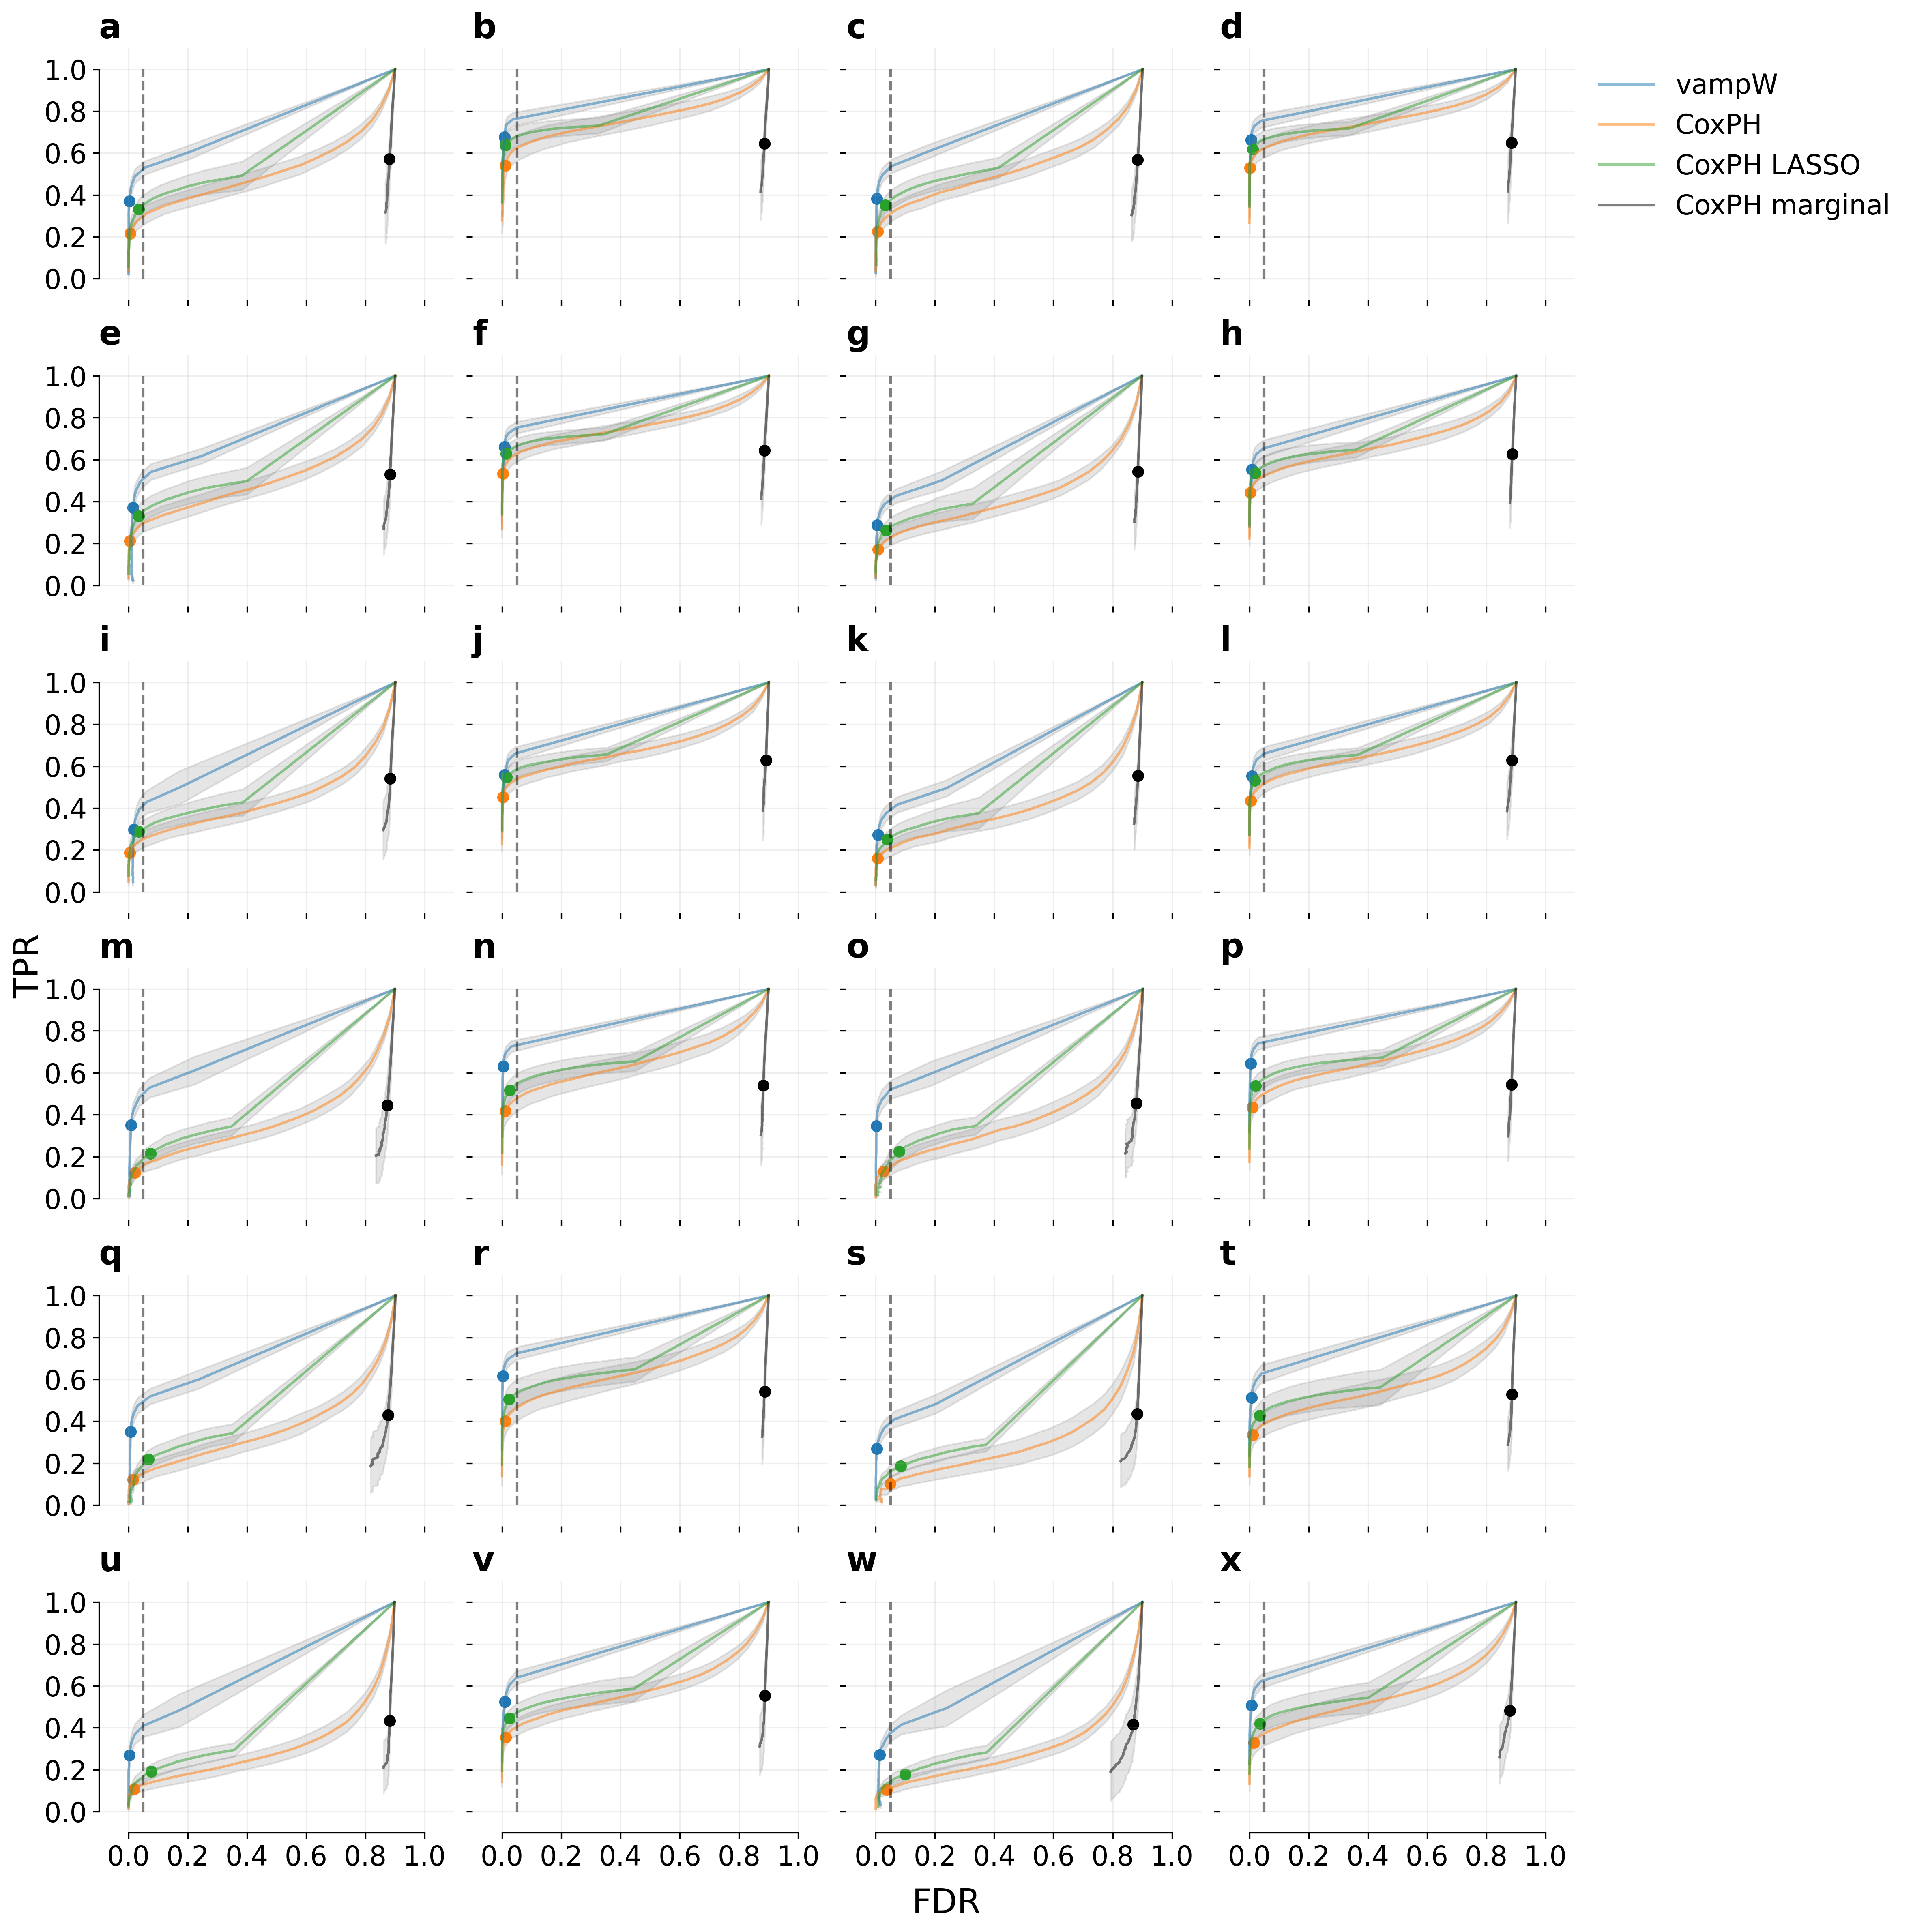
\includegraphics[width=\linewidth]{figures/sim_fdr_tpr.png}
    \end{center}
    \caption[Simulation study of variable selection performance using protein data from the UK Biobank]{\textbf{Simulation study of variable selection performance using protein data from the UK Biobank.} We simulate artificial phenotypic outcomes under 24 scenarios, corresponding to the parameterizations described in Supplementary Table \ref{tab:sim}, varying the proportion of variance explained, level of censoring, phenotype distribution, and distribution of regression coefficients. We compare the variable selection performance of vampW against several benchmarking methods (CoxPH, CoxPH LASSO and CoxPH marginal) in terms of the relationship between the false discovery rate (FDR) and true positive rate (TPR). For vampW, we use posterior inclusion probabilities (PIPs), with colored dots indicating a 0.95 threshold. For the other methods, p-value testing across multiple thresholds is employed, with colored dots indicating a Bonferroni-corrected 0.05 threshold.\label{fig:fdr_tpr}}
\end{figure}

\begin{figure}[H] % the continued legend, directly after the figure (on the next page)
    \ContinuedFloat
    \captionsetup{labelformat=continued}
    \caption[]{vampW maintains a calibrated FDR and consistently outperforms CoxPH-based models in TPR across all simulation scenarios, including those involving model misspecification. The error bars (gray shaded areas) represent the standard deviation across 50 simulation replicates.}
\end{figure}

\clearpage

\begin{figure}[H]
    \begin{center}
        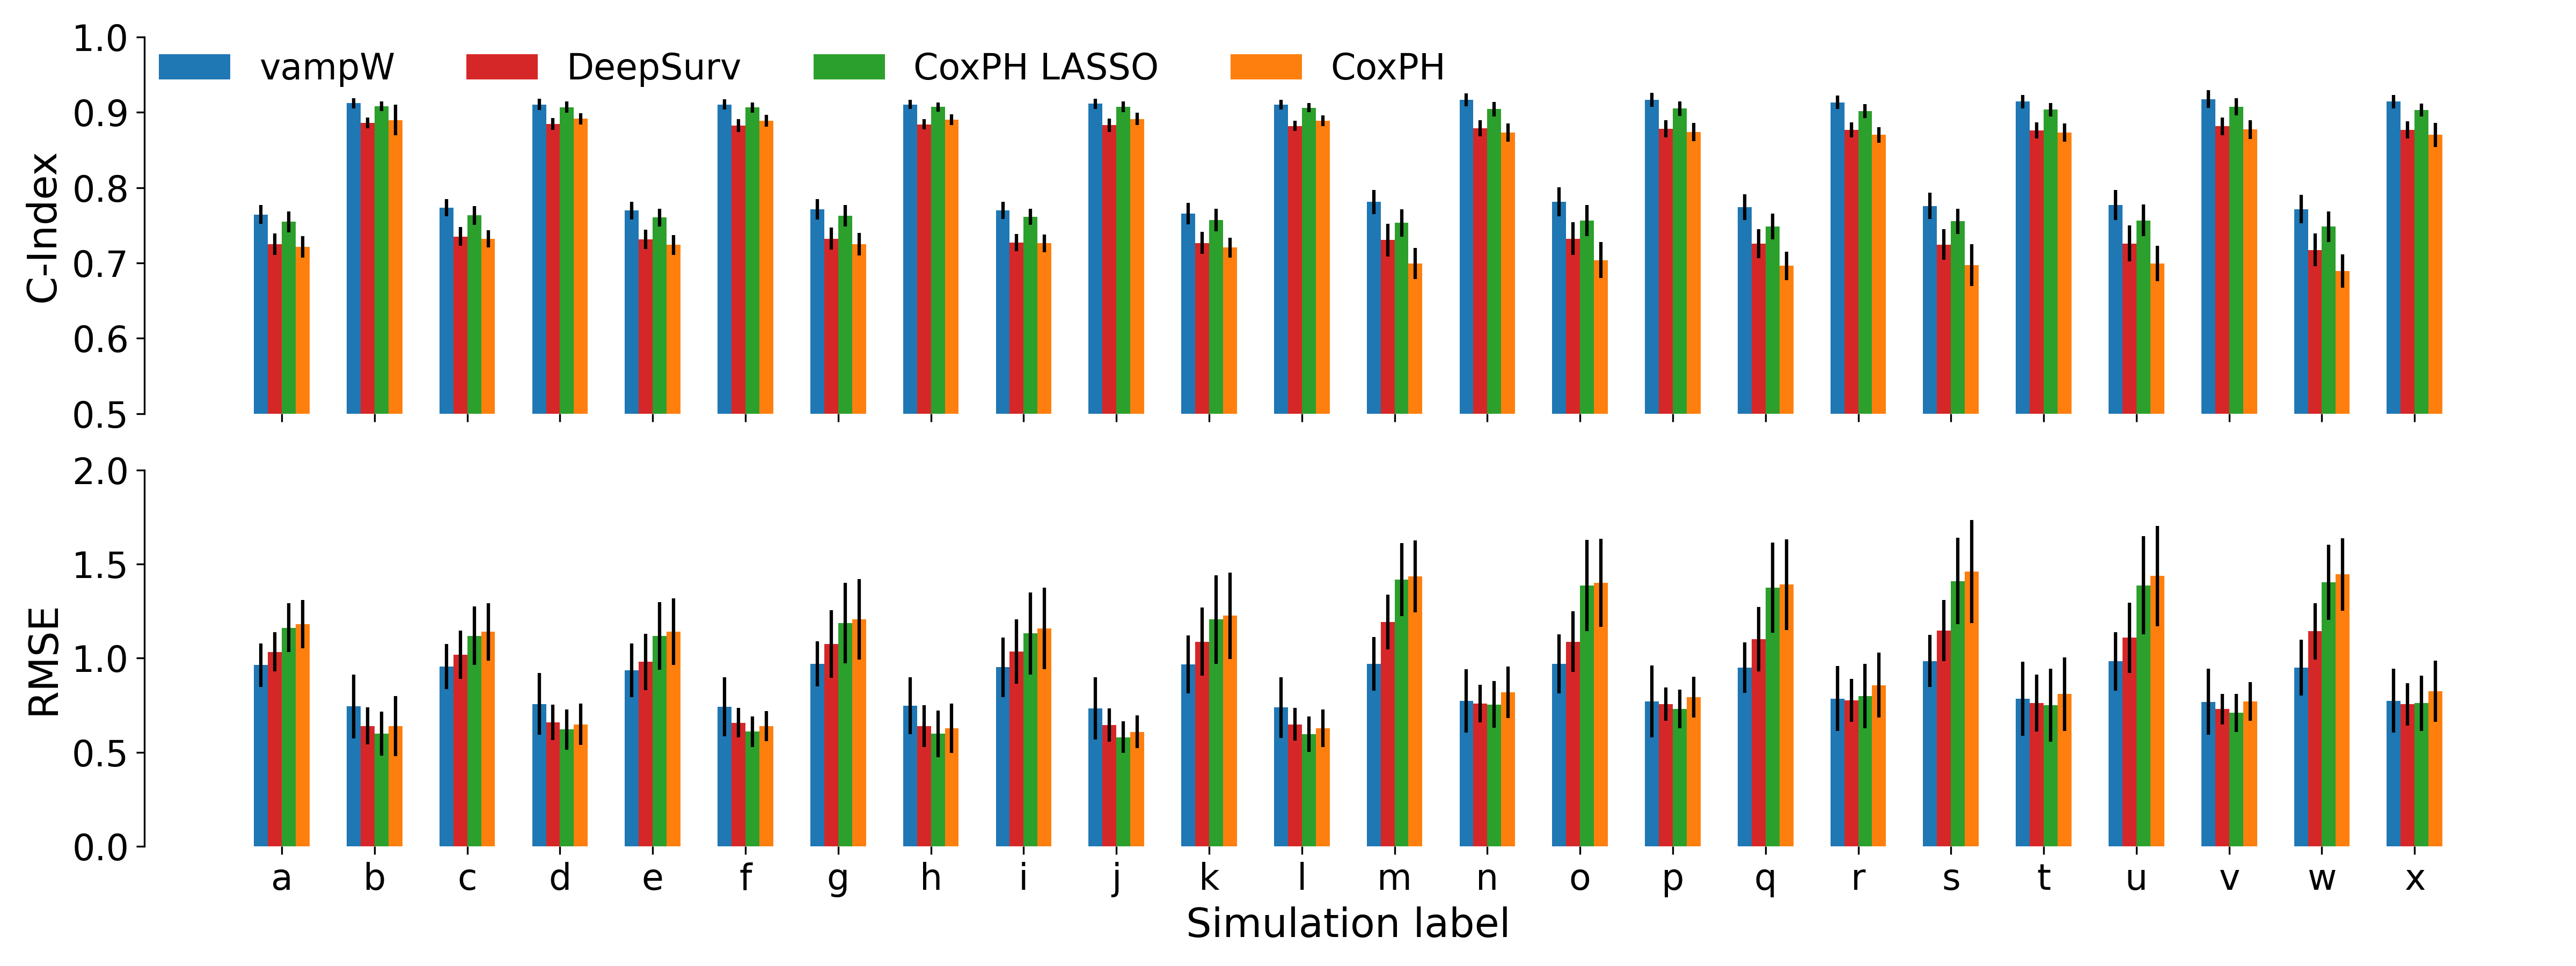
\includegraphics[width=\linewidth]{figures/sim_prediction.png}
    \end{center}
        \caption[Simulation study of out-of-sample prediction performance using protein data from the UK Biobank]{\textbf{Simulation study of out-of-sample prediction performance using protein data from the UK Biobank.} We evaluate predictive performance for time of onset across 24 simulated phenotypic outcomes corresponding to the parameterizations in Supplementary Table \ref{tab:sim}. We compare vampW with CoxPH, CoxPH LASSO, and DeepSurv in terms of concordance index (C-index) and root mean squared error (RMSE). The RMSE is evaluated in the logarithmic domain, assuming standardized outcomes with zero mean and unit variance. Across all simulated scenarios, vampW consistently demonstrates a clear improvement in the C-index when compared to both DeepSurv and the standard CoxPH model. When compared to CoxPH LASSO, the point estimate of C-index values for vampW improves, although it remains within overlapping error bars across all scenarios. In terms of RMSE, vampW strictly outperforms the standard CoxPH model in six scenarios and improves upon CoxPH LASSO in five scenarios. In all remaining comparisons, the predictive performance of the evaluated methods falls within each other's error margins. The reported error bars represent the standard deviation across 50 simulation replicates (black lines at the top of the colored bars). 
        \label{fig:sim_prediction}}
\end{figure}

\clearpage


\begin{figure}[H]
\begin{center}
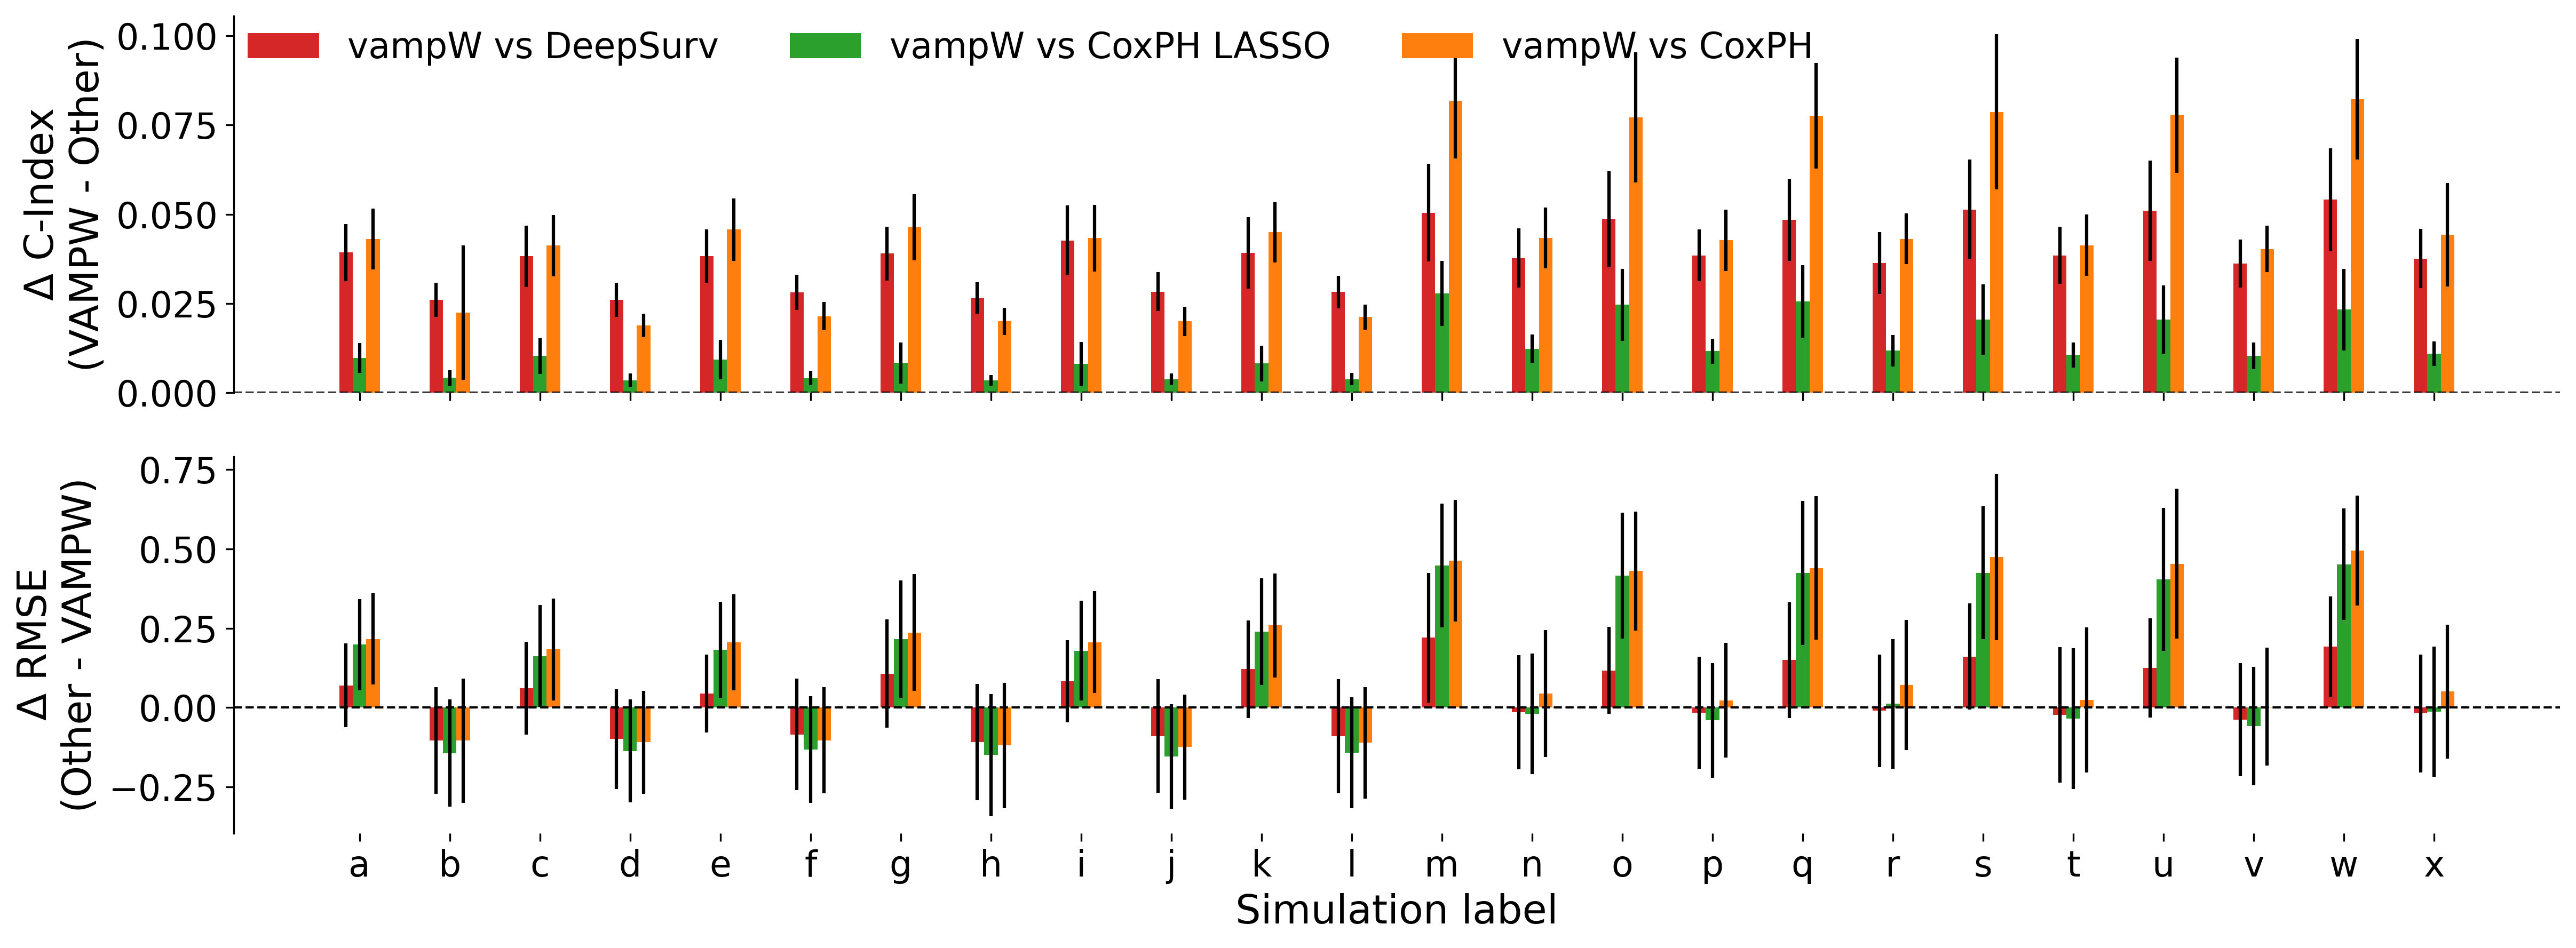
\includegraphics[width=\linewidth]{figures/sim_paired_differences.png}
\end{center}
% \caption{\textbf{Paired differences in out-of-sample prediction performance across simulated phenotypic outcomes.} We evaluate predictive performance of vampW compared to DeepSurv, CoxPH LASSO, and the standard CoxPH model across 24 simulated scenarios (corresponding to the parameterizations in Table \ref{tab:sim}). The top panel displays the paired difference in concordance index ($\Delta$ C-index), calculated as VAMPW minus the competing method. The bottom panel shows the paired difference in root mean squared error ($\Delta$ RMSE), calculated as the competing method minus VAMPW. By this formulation, consistent positive values in both panels (bars extending above the dashed zero line) would indicate superior predictive performance of vampW compared to other benchmarking methods. The RMSE is evaluated in the logarithmic domain, assuming standardized outcomes with zero mean and unit variance. The reported error bars represent the standard deviation of the paired differences across 50 simulation replicates (black lines at the top or bottom of the colored bars). In terms of C-index vampW, paired difference with error bars never crosses zero threshold indicating that vampW is outperforming other methods across all scenarios.  In terms of RMSE, vampW is always on par with the competitor methods or outperforming them.
% \label{fig:sim_paired_differences}}
% \end{figure}
\caption[Paired differences in out-of-sample prediction performance across simulated phenotypic outcomes]{\textbf{Paired differences in out-of-sample prediction performance across simulated phenotypic outcomes.} We evaluate the predictive performance of vampW compared to DeepSurv, CoxPH LASSO, and the standard CoxPH model across 24 simulated scenarios (corresponding to the parameterizations in Supplementary Table \ref{tab:sim}). The top panel displays the paired difference in concordance index ($\Delta$ C-index), calculated as vampW minus the competing method. The bottom panel shows the paired difference in root mean squared error ($\Delta$ RMSE), calculated as the competing method minus vampW. By this formulation, positive values in both panels (bars extending above the dashed zero line) indicate superior predictive performance by vampW. The RMSE is evaluated in the logarithmic domain, assuming standardized outcomes with zero mean and unit variance. The reported error bars represent the standard deviation of the paired differences across 50 simulation replicates (black lines at the top or bottom of the colored bars). For the C-index, the paired differences, inclusive of error bars, never cross the zero threshold, indicating that vampW consistently outperforms the other methods across all scenarios. In terms of RMSE, vampW achieves performance that is either on par with or superior to the competing methods.
}
\label{fig:sim_paired_differences}
\end{figure}

\clearpage

\begin{figure}[H]
    \begin{center}
        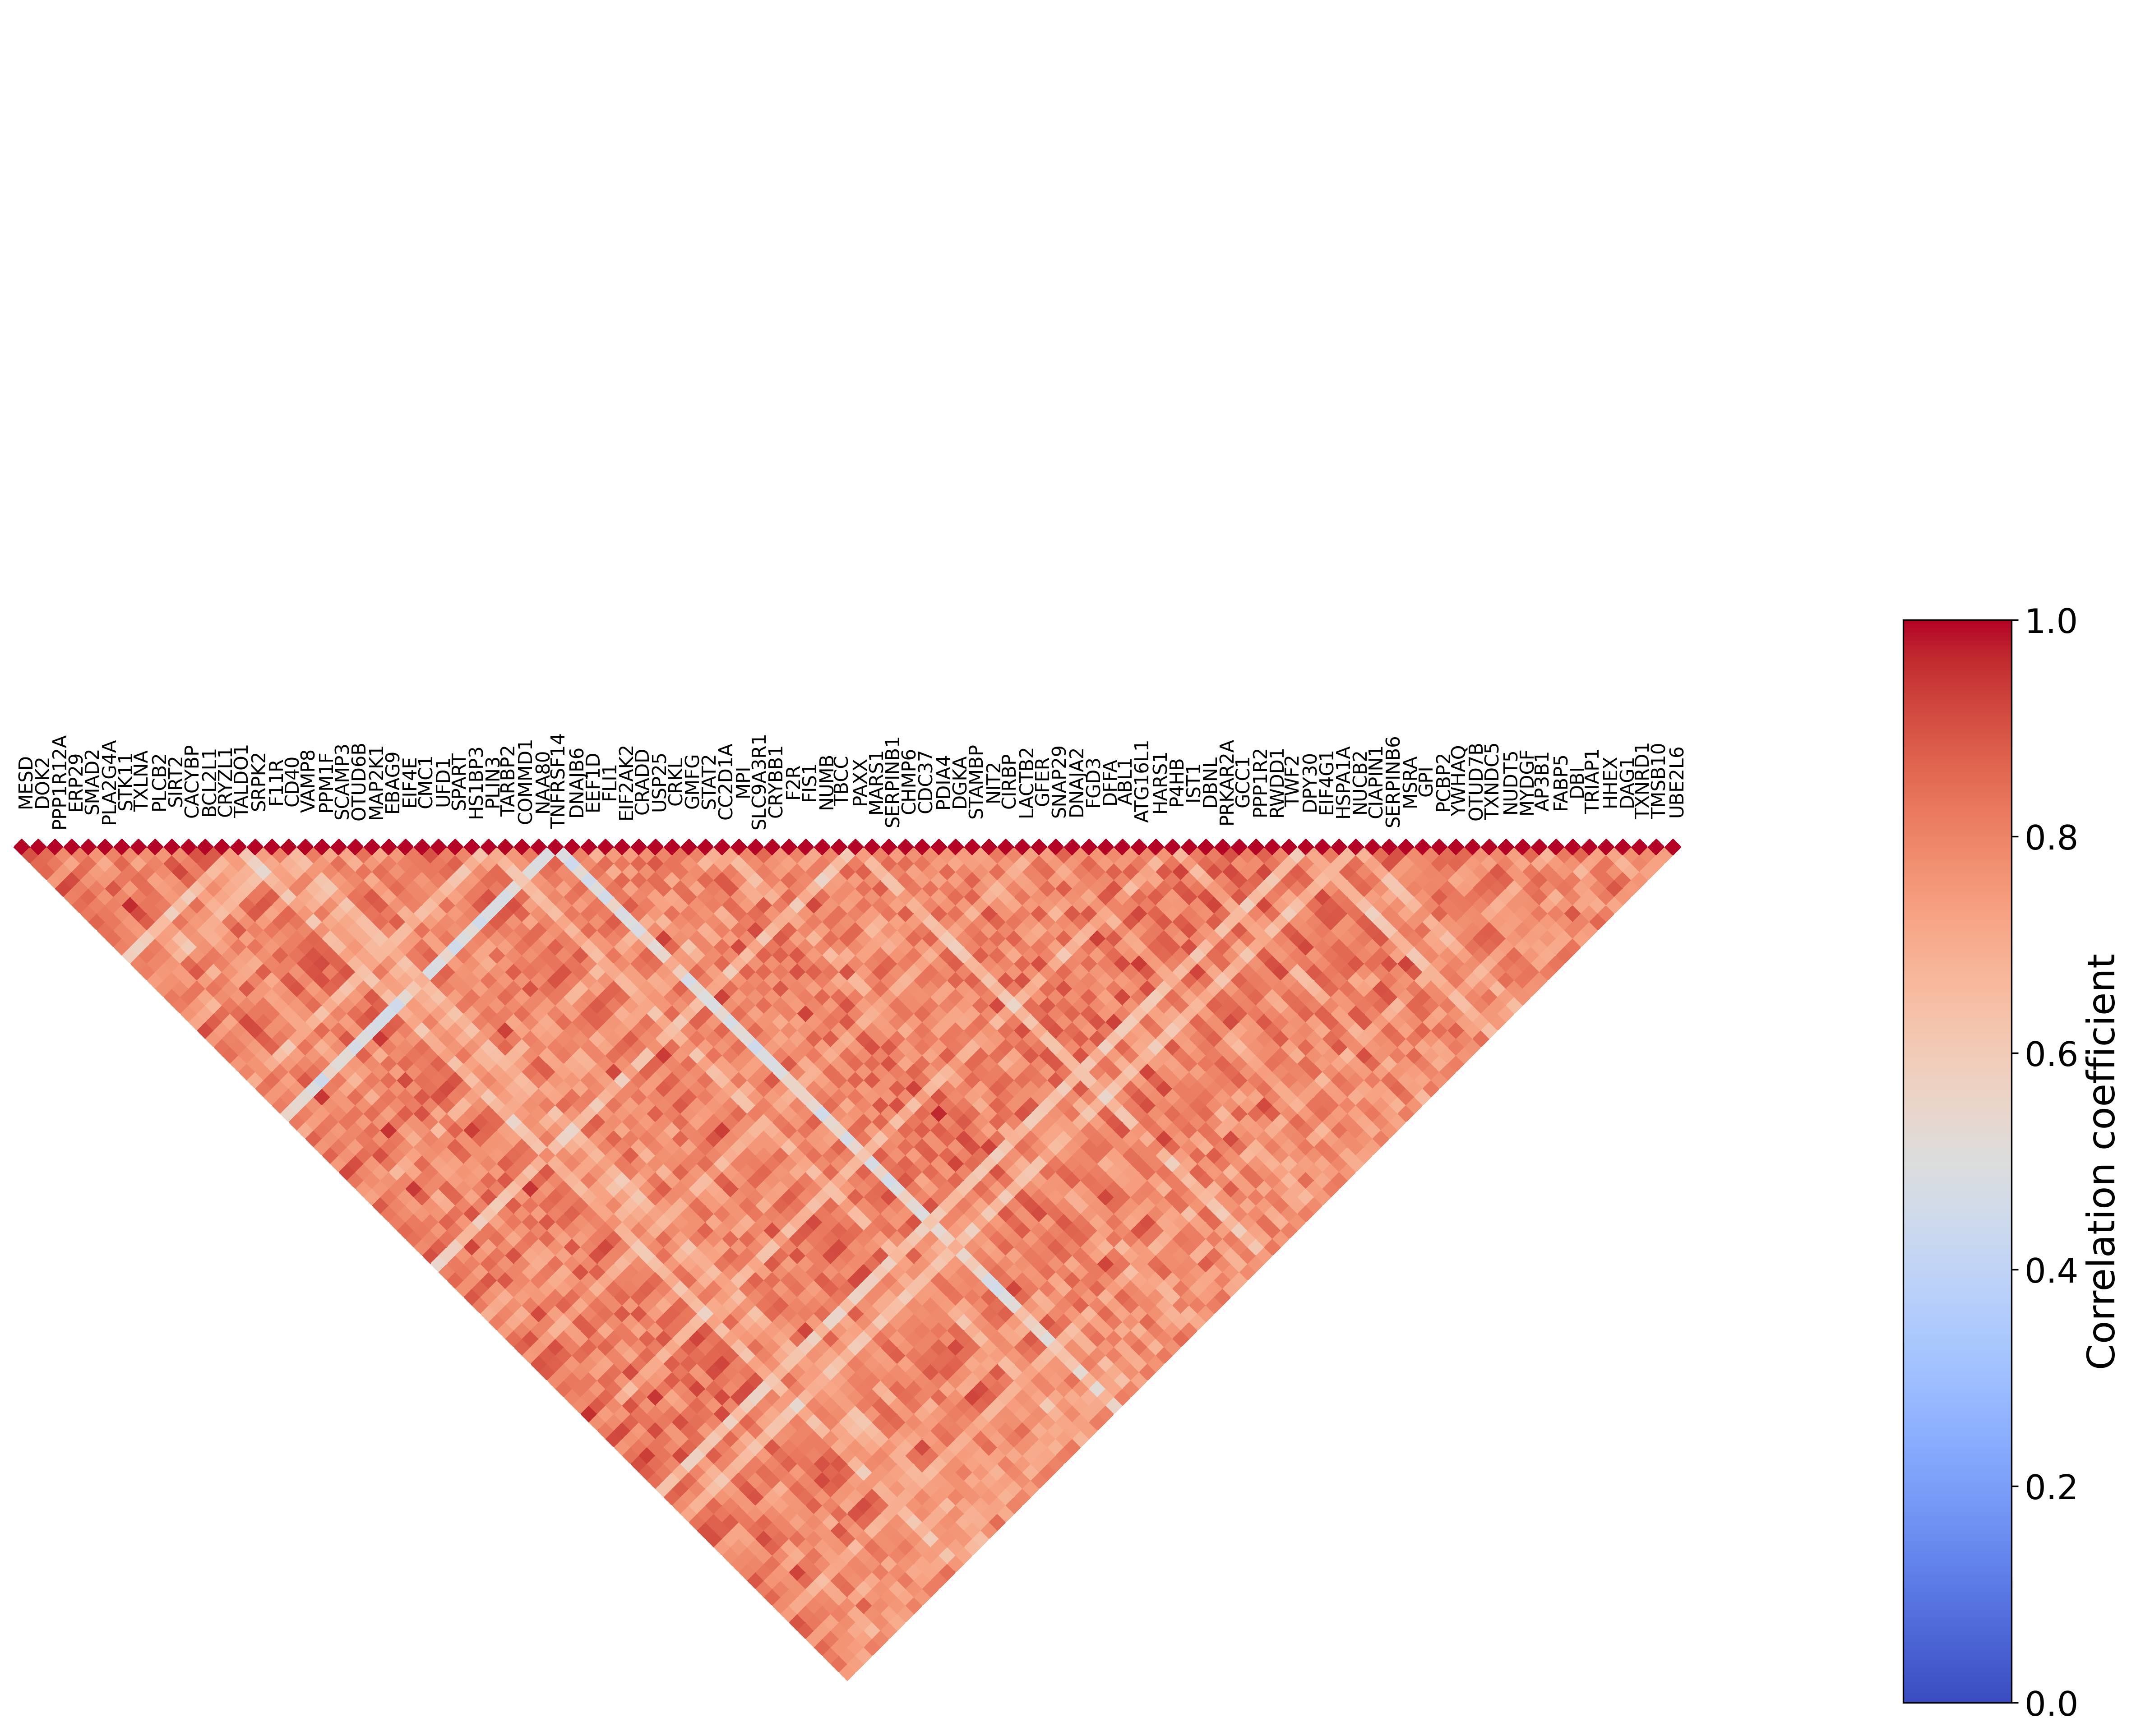
\includegraphics[width=\linewidth]{figures/corr_mat.png}
    \end{center}
    \caption[Correlation structure of the protein measures in the UK Biobank]{\textbf{Correlation structure of the protein measures in the UK Biobank.} We calculate Pearson product-moment correlation coefficients for all proteins, not-adjusted for covariates, and select the top 100 most correlated ones. We plot the correlation structure along with corresponding protein-coding genes.\label{fig:correlation}}
\end{figure}

\clearpage

\begin{figure}[H]
    \begin{center}
        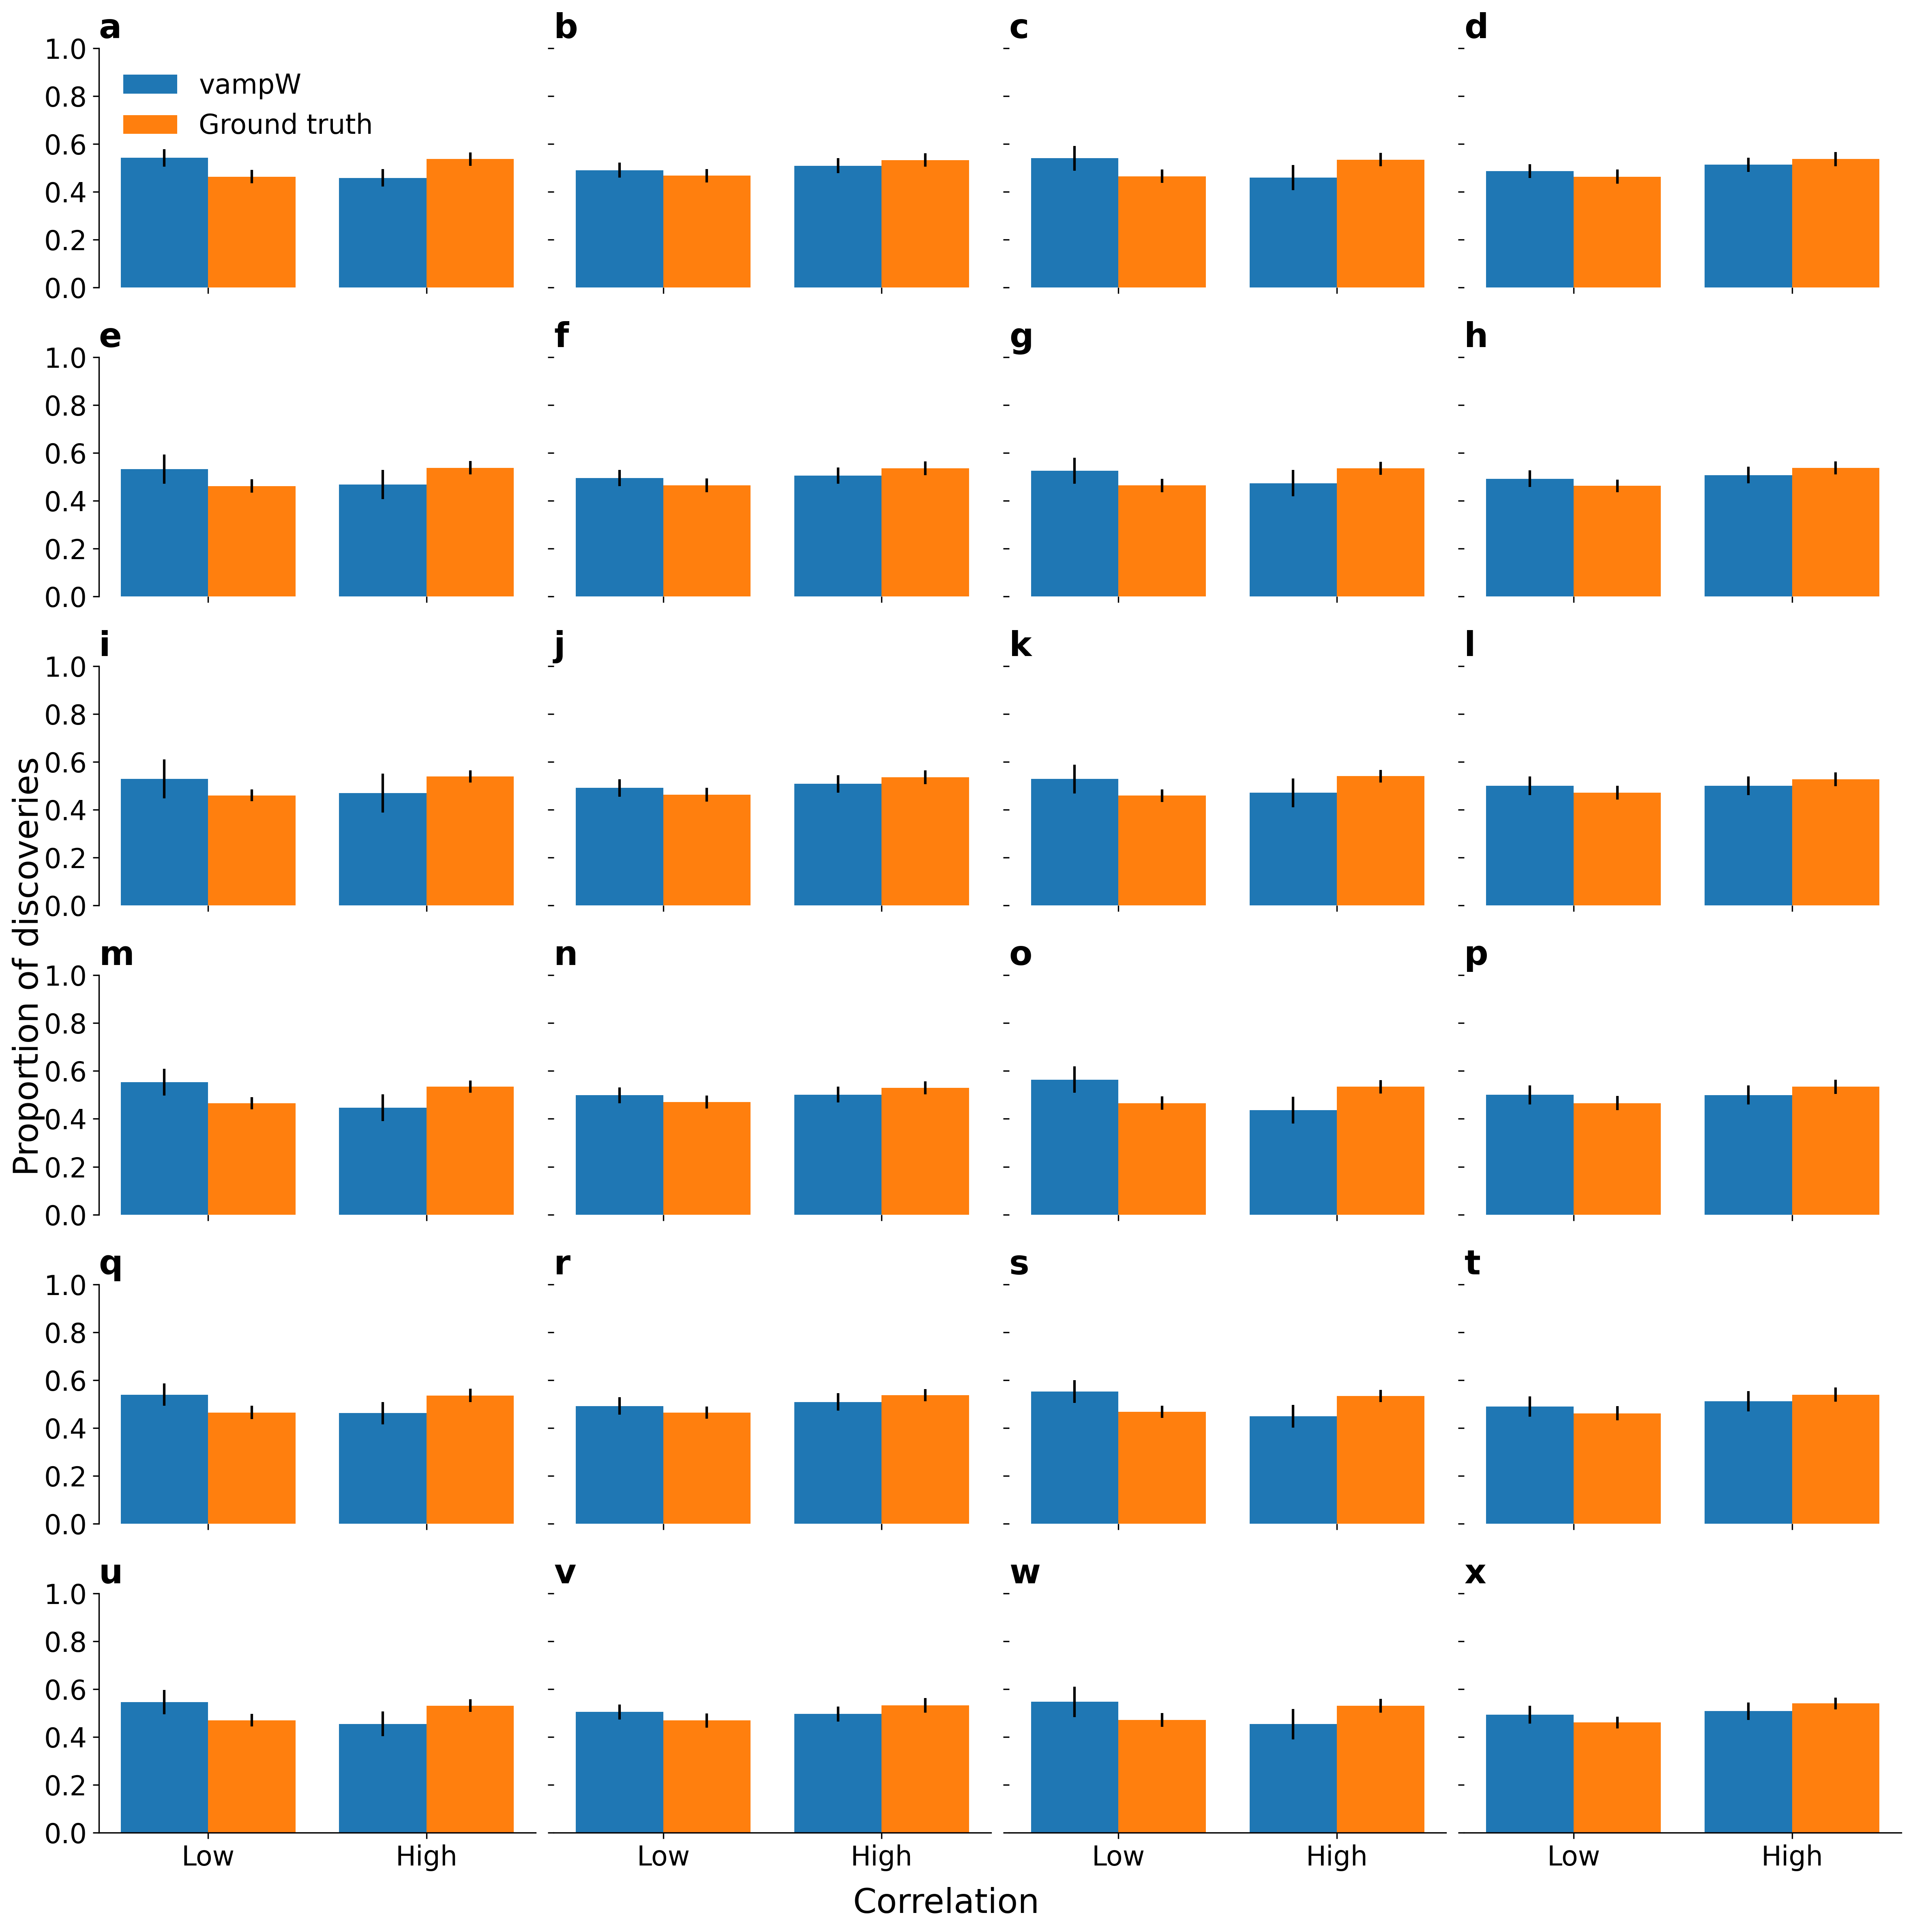
\includegraphics[width=\linewidth]{figures/sim_annot.png}
    \end{center}
    \caption[Protein annotation based on correlation structure]{\textbf{Protein annotation based on correlation structure}. For 24 simulation scenarios, described in Supplementary Table \ref{tab:sim}, we visualize the relative proportion of highly and low-correlated true positive discoveries with respect to all true positive discoveries (blue), and compare this to the proportion of highly and low-correlated causal proteins with respect to all causal proteins (orange). If the correlation of a particular protein with any other protein is greater than 0.5 (absolute value of Pearson correlation coefficient), it is categorized as a highly correlated protein. The remaining proteins are categorized as low-correlated. The black bars show 1 standard error over 50 simulation replicas. The results suggest that vampW detects causal signals even for proteins with correlations above the 0.5 threshold.
\label{fig:annot}}
\end{figure}

\clearpage

\begin{figure}[H]
    \begin{center}
        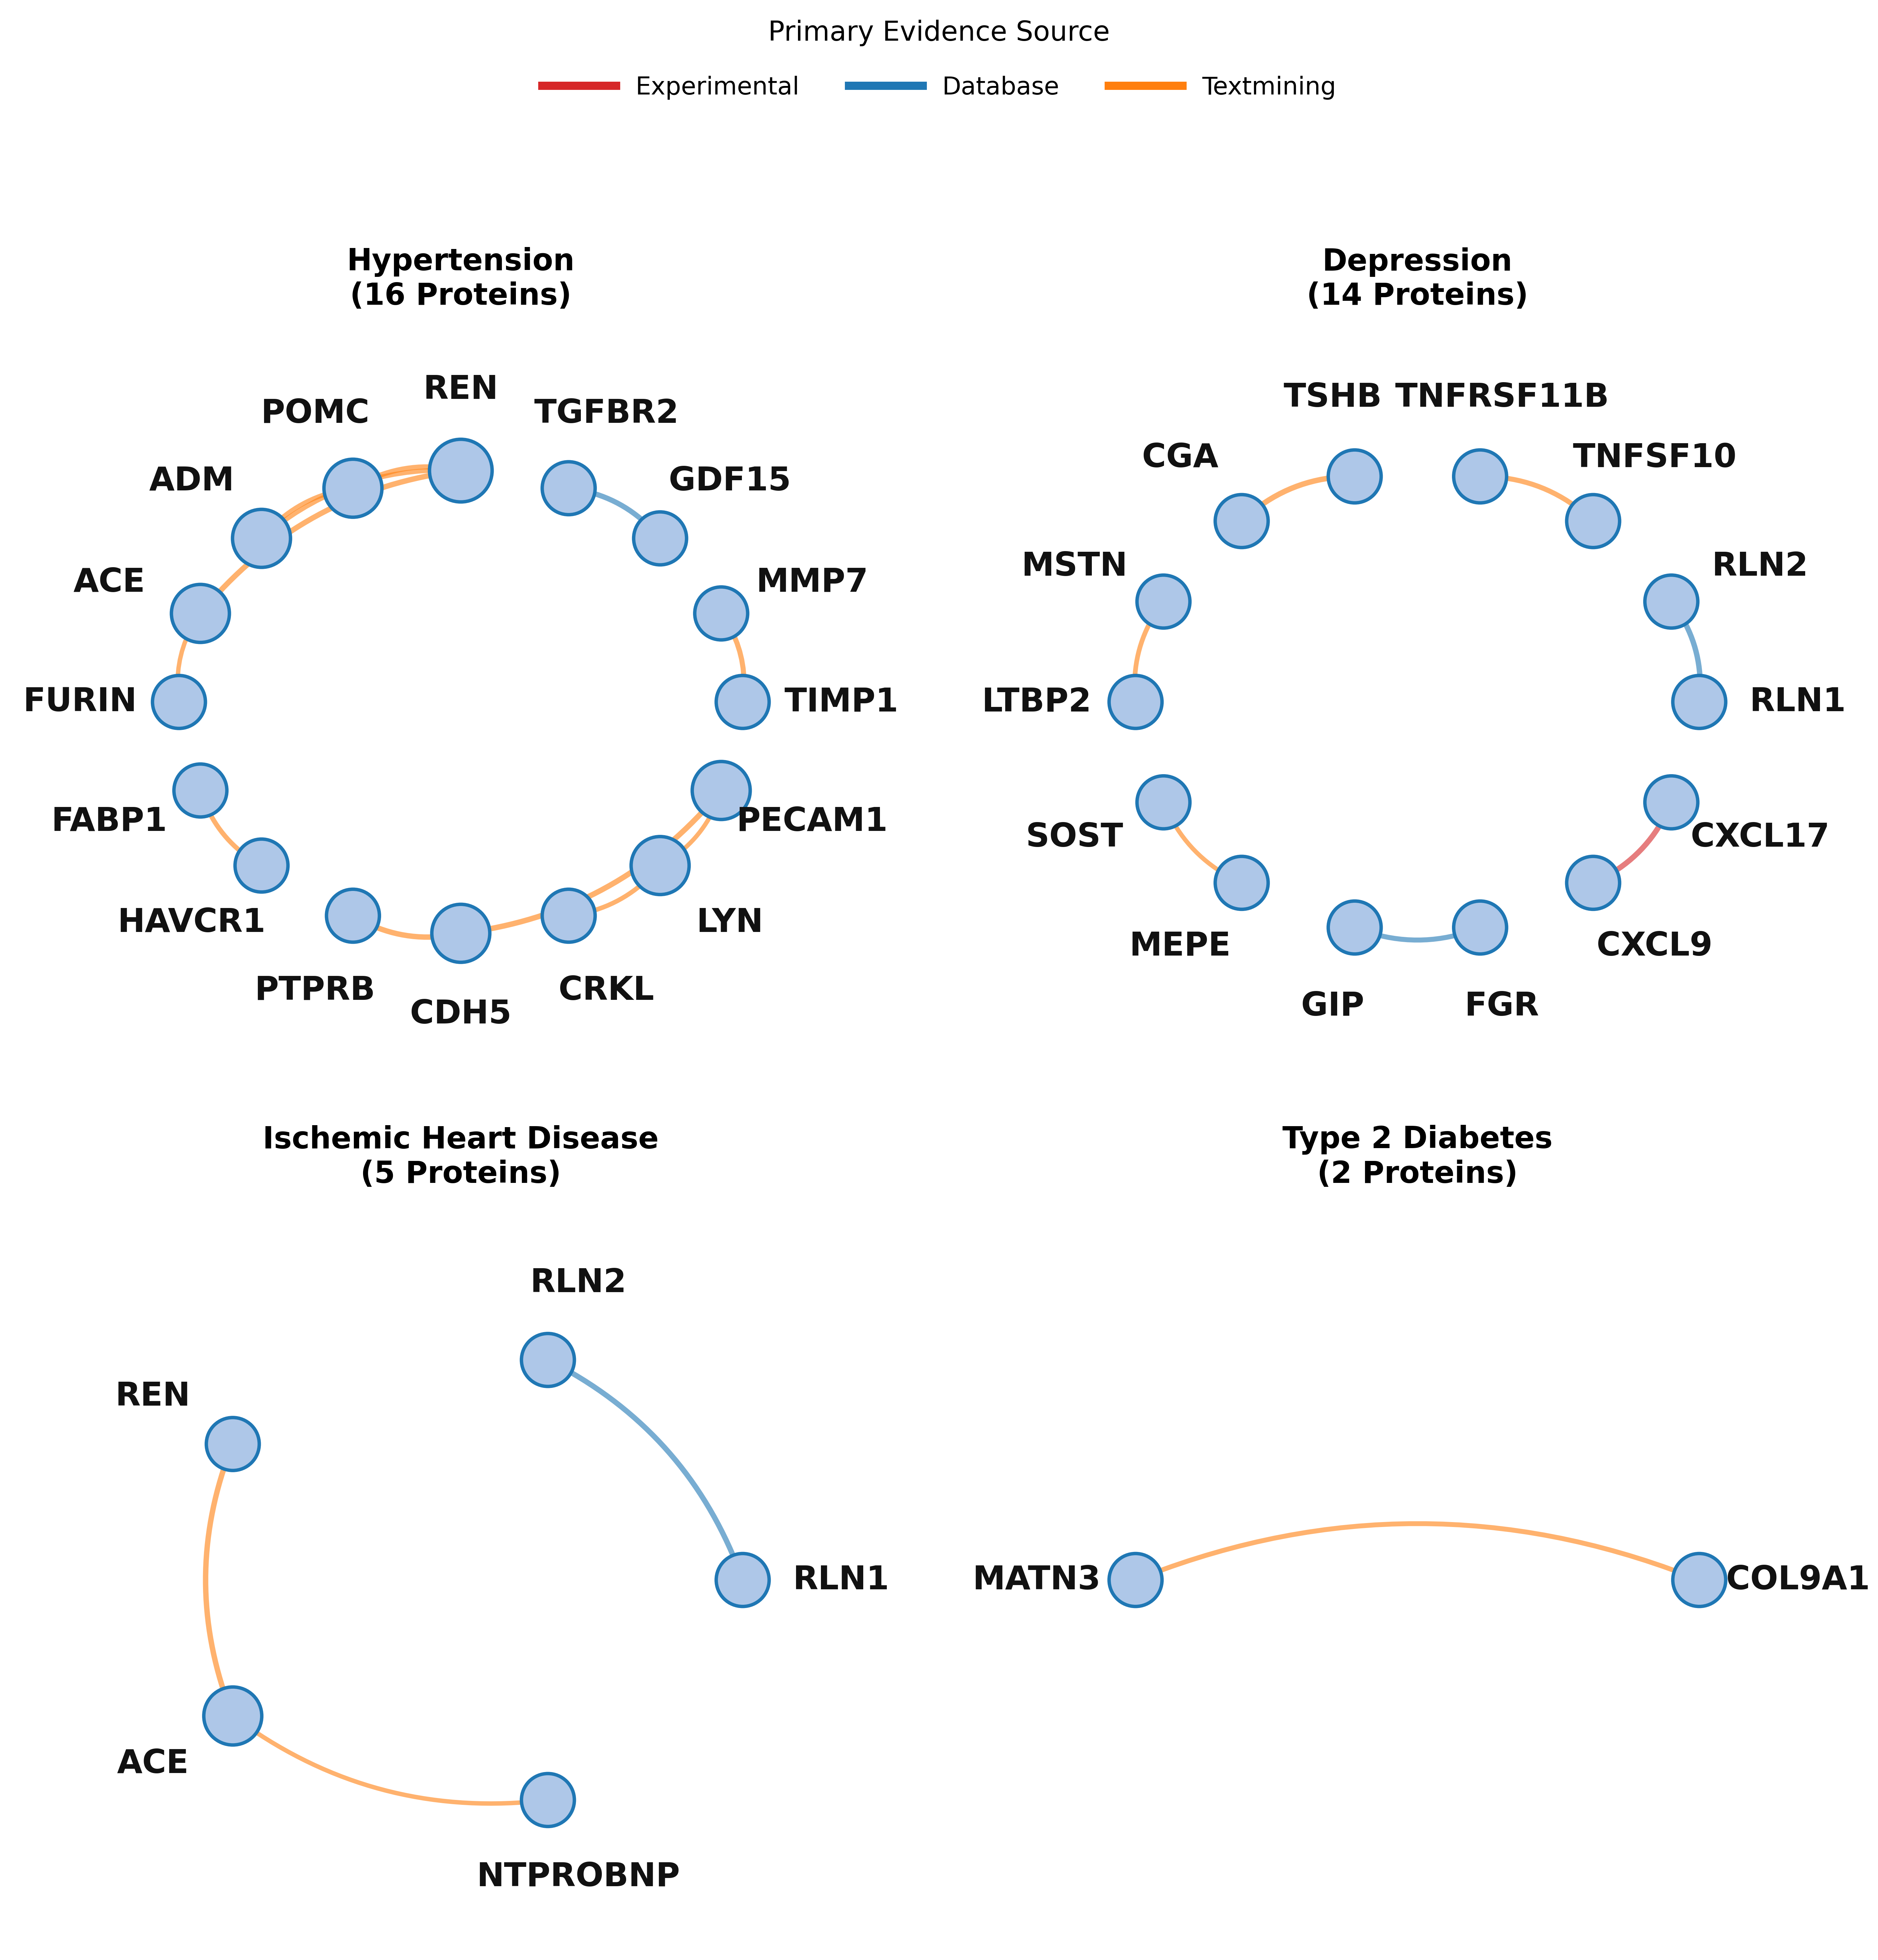
\includegraphics[width=\linewidth]{figures/summary_panel_plot.png}
    \end{center}
    \caption[Protein-protein interaction networks for trait-associated proteins]{\textbf{Protein-protein interaction networks for trait-associated proteins.} Network visualizations of significant proteins associated with Hypertension, Depression, Ischemic Heart Disease, and Type 2 Diabetes. Nodes represent individual proteins identified in the analysis. Edges denote known interactions retrieved from the STRING database (version 12.0), filtered for high-confidence connections (combined score $\ge 800$). Edge colors indicate the primary source of evidence supporting the interaction: experimental validation (red), curated databases (blue), or automated text mining (orange). Node sizes are proportionally scaled by their degree (number of connections) within the local trait network. Proteins without high-confidence interactions in the selected sub-network are excluded from the visualization.}\label{fig:interaction_networks}

\end{figure}

\clearpage

\begin{figure}[H]
    \begin{center}
        \includegraphics[width=\linewidth]{figures/cov_lin_exp.png}
    \end{center}
    \caption[Adjusting for non-linear effects of age on protein levels]{\textbf{Adjusting for non-linear effects of age on protein levels}.  In addition to the standard linear adjustment (blue) for the age covariate, we evaluate the vampW model using protein data adjusted for exponential age effects (orange). In column (a), we show significant protein-coding genes at their corresponding DNA positions that pass a PIP threshold of 0.95 for four representative outcomes, namely Alzheimer's disease, ischemic heart disease, colorectal cancer, and death. In column (b), we show the relationship between PIPs passing a threshold of 0.9 across the two models, where PIP$_{lin}$ and PIP$_{exp}$ denote the standard linear and exponential age adjustments, respectively. Notably, the gene \emph{CGA}, previously reported as age-associated in recent work, disappears from the discoveries when considering non-linear effects of age on protein levels.
\label{fig:cov_age}}
\end{figure}

\clearpage

\begin{figure}[H]
    \begin{center}
        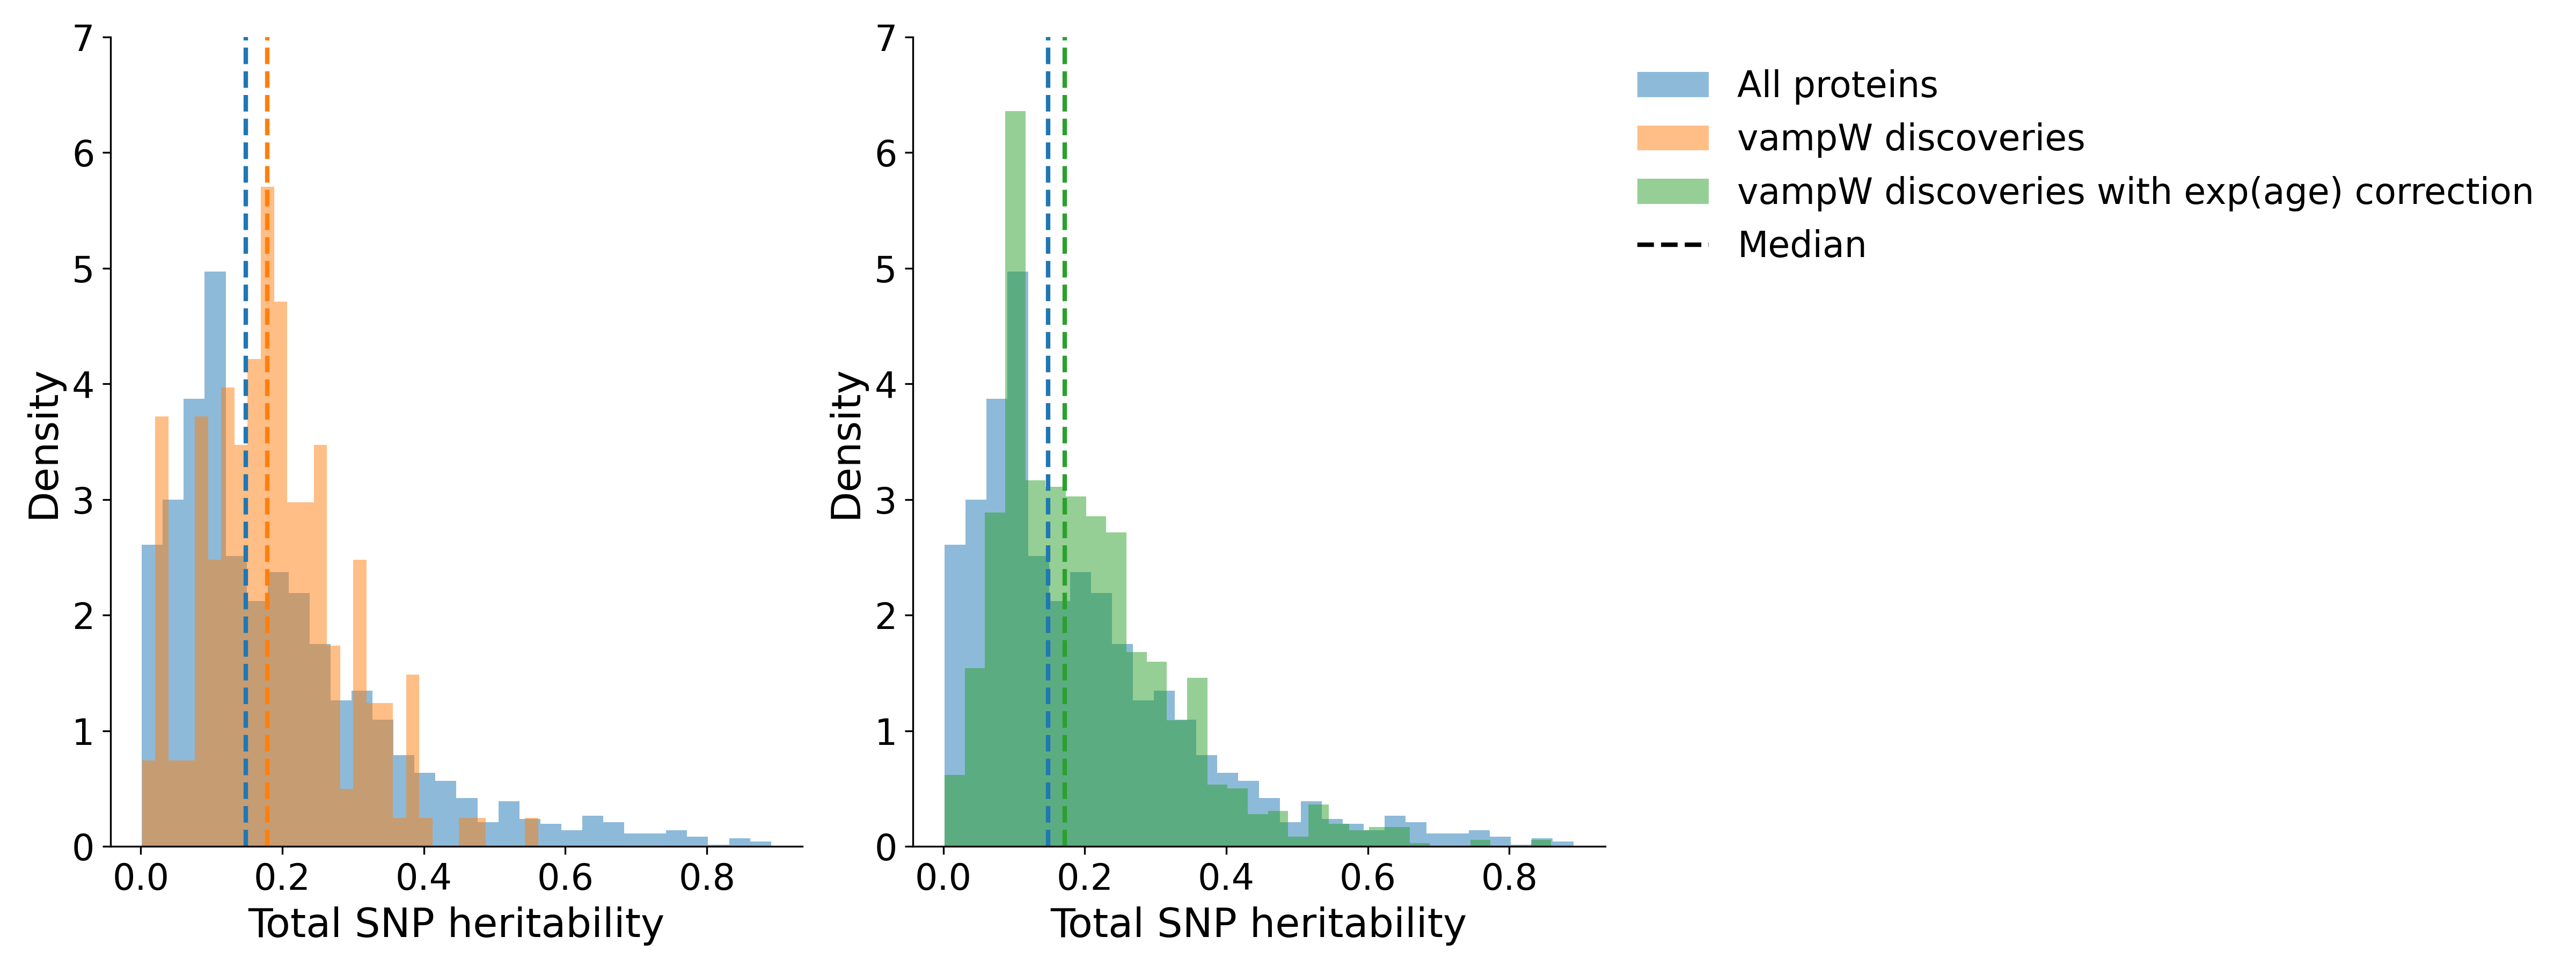
\includegraphics[width=\linewidth]{figures/protein_h2.png}
    \end{center}
    \caption[Distribution of total SNP-based heritability of proteins with pQTLs]{\changed{\textbf{Distribution of total SNP-based heritability of proteins with pQTLs.} We plot the distributions of total SNP heritability for 2,430 proteins reported in the study \cite{sun_plasma_2023}, including all proteins with pQTLs (blue) and the corresponding subset overlapping with vampW discoveries, with (green) and without (orange) exponential age correction. The vampW discoveries exhibit average heritability of 19.9\% and 18.7\% for models with and without exponential age correction, respectively, compared to a mean heritability of 19.5\% across all proteins with pQTLs.}}\label{fig:protein_h2}
\end{figure}

\clearpage

\begin{figure}[H]
    \begin{center}
        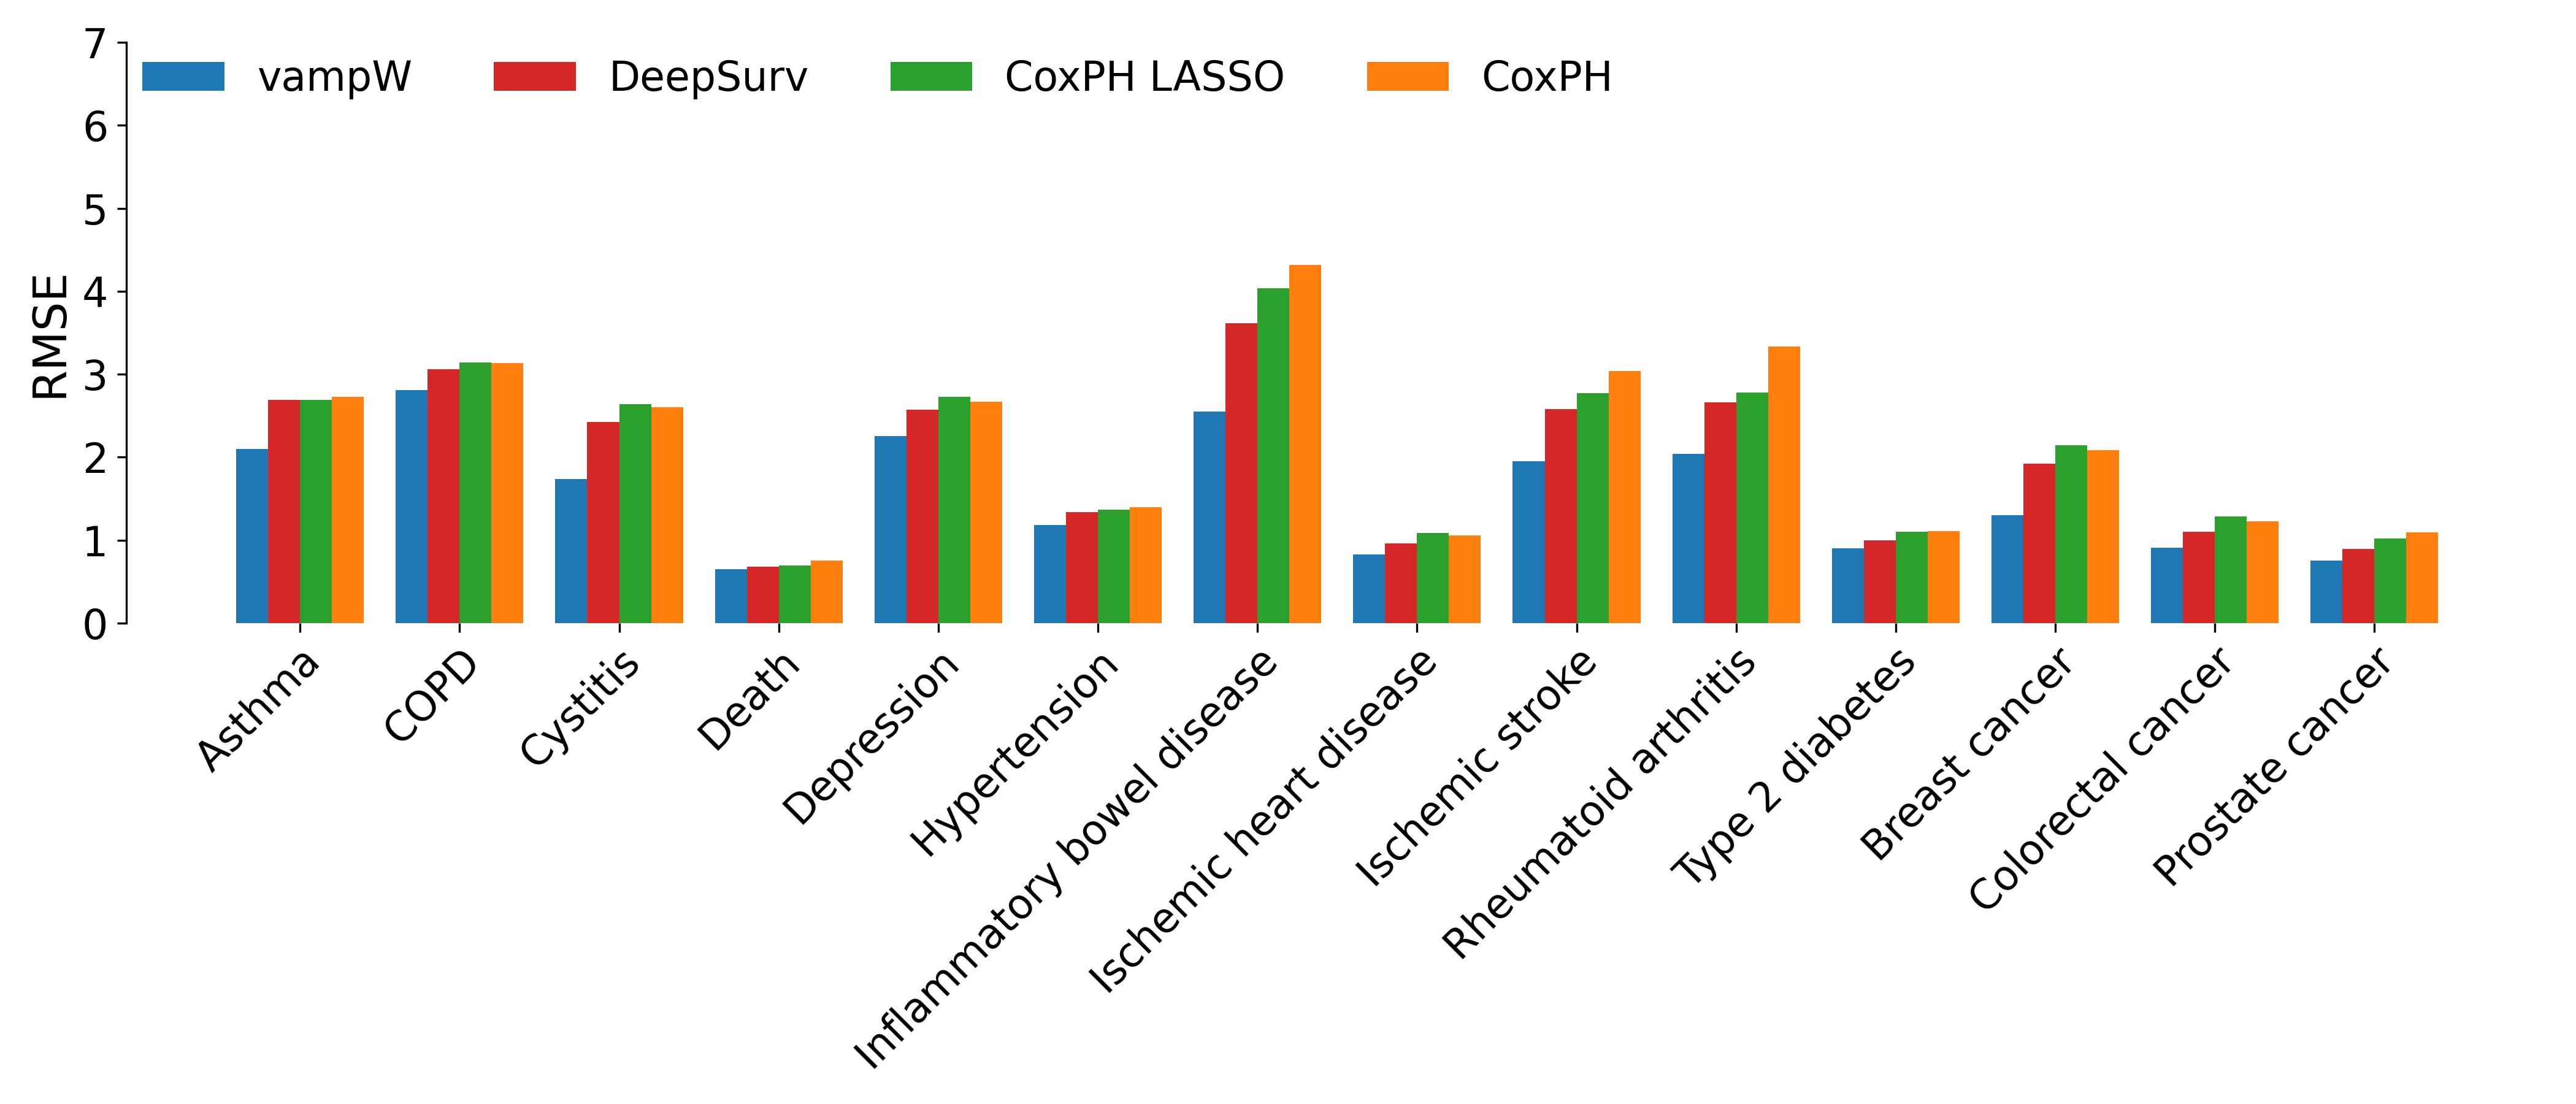
\includegraphics[width=\linewidth]{figures/real_rmse_time.png}
    \end{center}
    \caption[Out-of-sample performance comparison in terms of RMSE on the log-normalized times for CoxPH, LASSO-penalized CoxPH, DeepSurv, and vampW]{\textbf{Out-of-sample performance comparison in terms of RMSE on the log-normalized times for CoxPH, LASSO-penalized CoxPH, DeepSurv, and vampW.}
    We evaluate time-to-diagnosis predictions for 14 health-related outcomes in the UK Biobank (traits with $\ge 100$ cases present in the test set) using protein measurements adjusted for age and sex. % using linear regression approach. 
    The accuracy of the model is assessed using the root mean squared error (RMSE). The training is performed on data that is first log-transformed and standardized to zero mean and unit variance, and then scaled back using an exponential transformation. The RMSE calculation presented in this figure is performed on the logarithmic scale in which the data is standardized, and it includes only uncensored individuals across traits.}
\label{fig:real_rmse_time}
\end{figure}

\clearpage 

\begin{figure}[H]
    \begin{center}
        \includegraphics[width=1.0\linewidth]{figures/weibull_fits_dedup.png}
    \end{center}
    \caption[Analysis of age-at-onset distributions for UK Biobank traits]{\textbf{Analysis of age-at-onset distributions for UK Biobank traits}. The histograms display the empirical distribution of age-at-onset for cases across various phenotypes in the training set. The blue bars represent the density of observed onset ages, while the solid red line indicates the fitted Weibull probability density function (PDF). Outliers were excluded from the fitting process using the Interquartile Range (IQR) method. The title of each subplot provides goodness-of-fit metrics, including the Kolmogorov-Smirnov statistic (KS), Wasserstein distance (W), and Total Variation distance (TV). \label{fig:distance} } %Additionally, the percentage of "prospective drops" is reported, indicating the proportion of cases where the age of onset occurred after the baseline assessment.}
\end{figure}

\clearpage

\begin{figure}[H]
    \begin{center}
        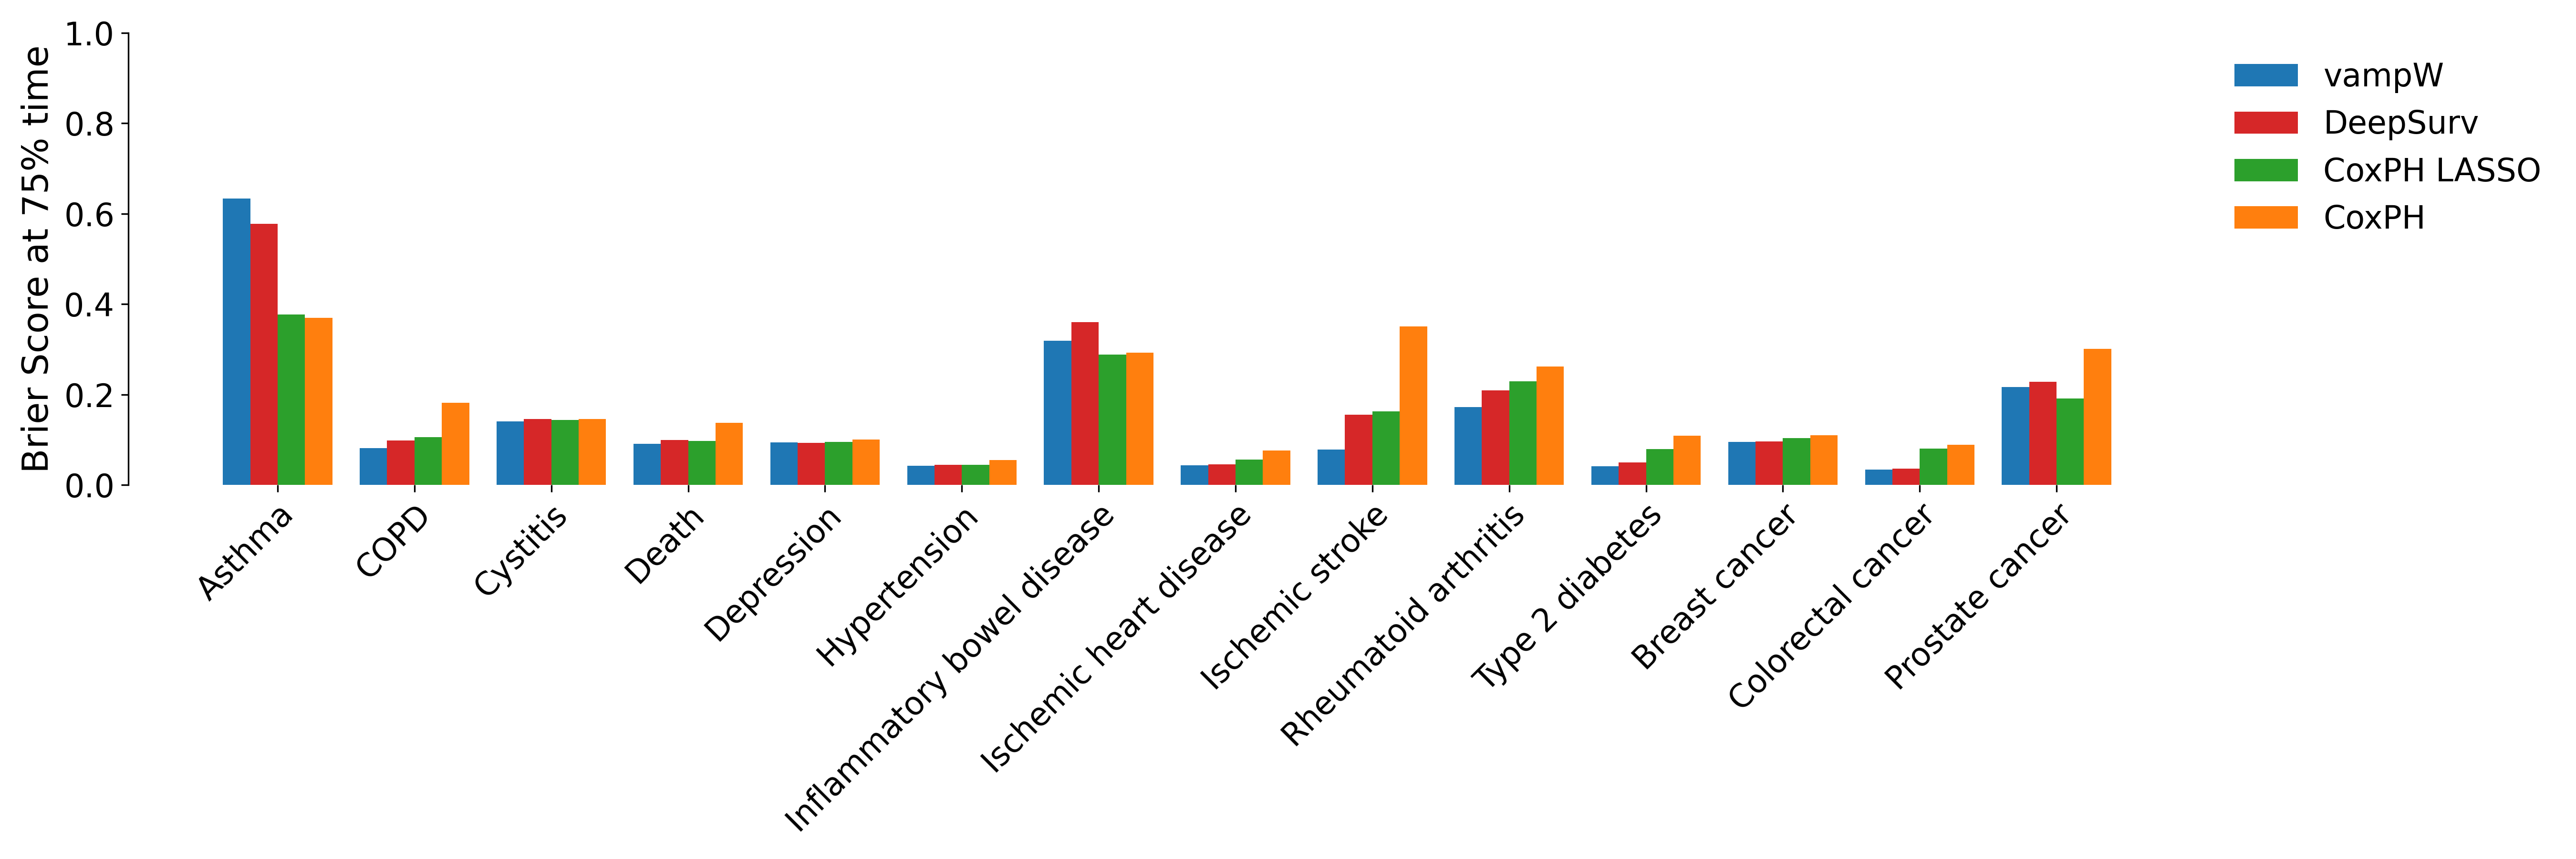
\includegraphics[width=\linewidth]{figures/bs_t75.png}
    \end{center}
    \caption[Brier Score comparison across methods evaluated at the 75\% time point]{\textbf{Brier Score comparison across methods evaluated at the 75\% time point.} We calculate the Brier Score (BS), a standard metric for evaluating the out-of-sample performance of time-to-event predictions. We report the BS value at the time corresponding to 75\% of the time span within the observed time period. Among 14 UK Biobank outcomes with sufficient sample size for out-of-sample evaluation, vampW outperforms the other benchmarking methods in 10 cases.}\label{fig:bs_t75}
\end{figure}

\clearpage

\begin{figure}[H]
    \begin{center}
        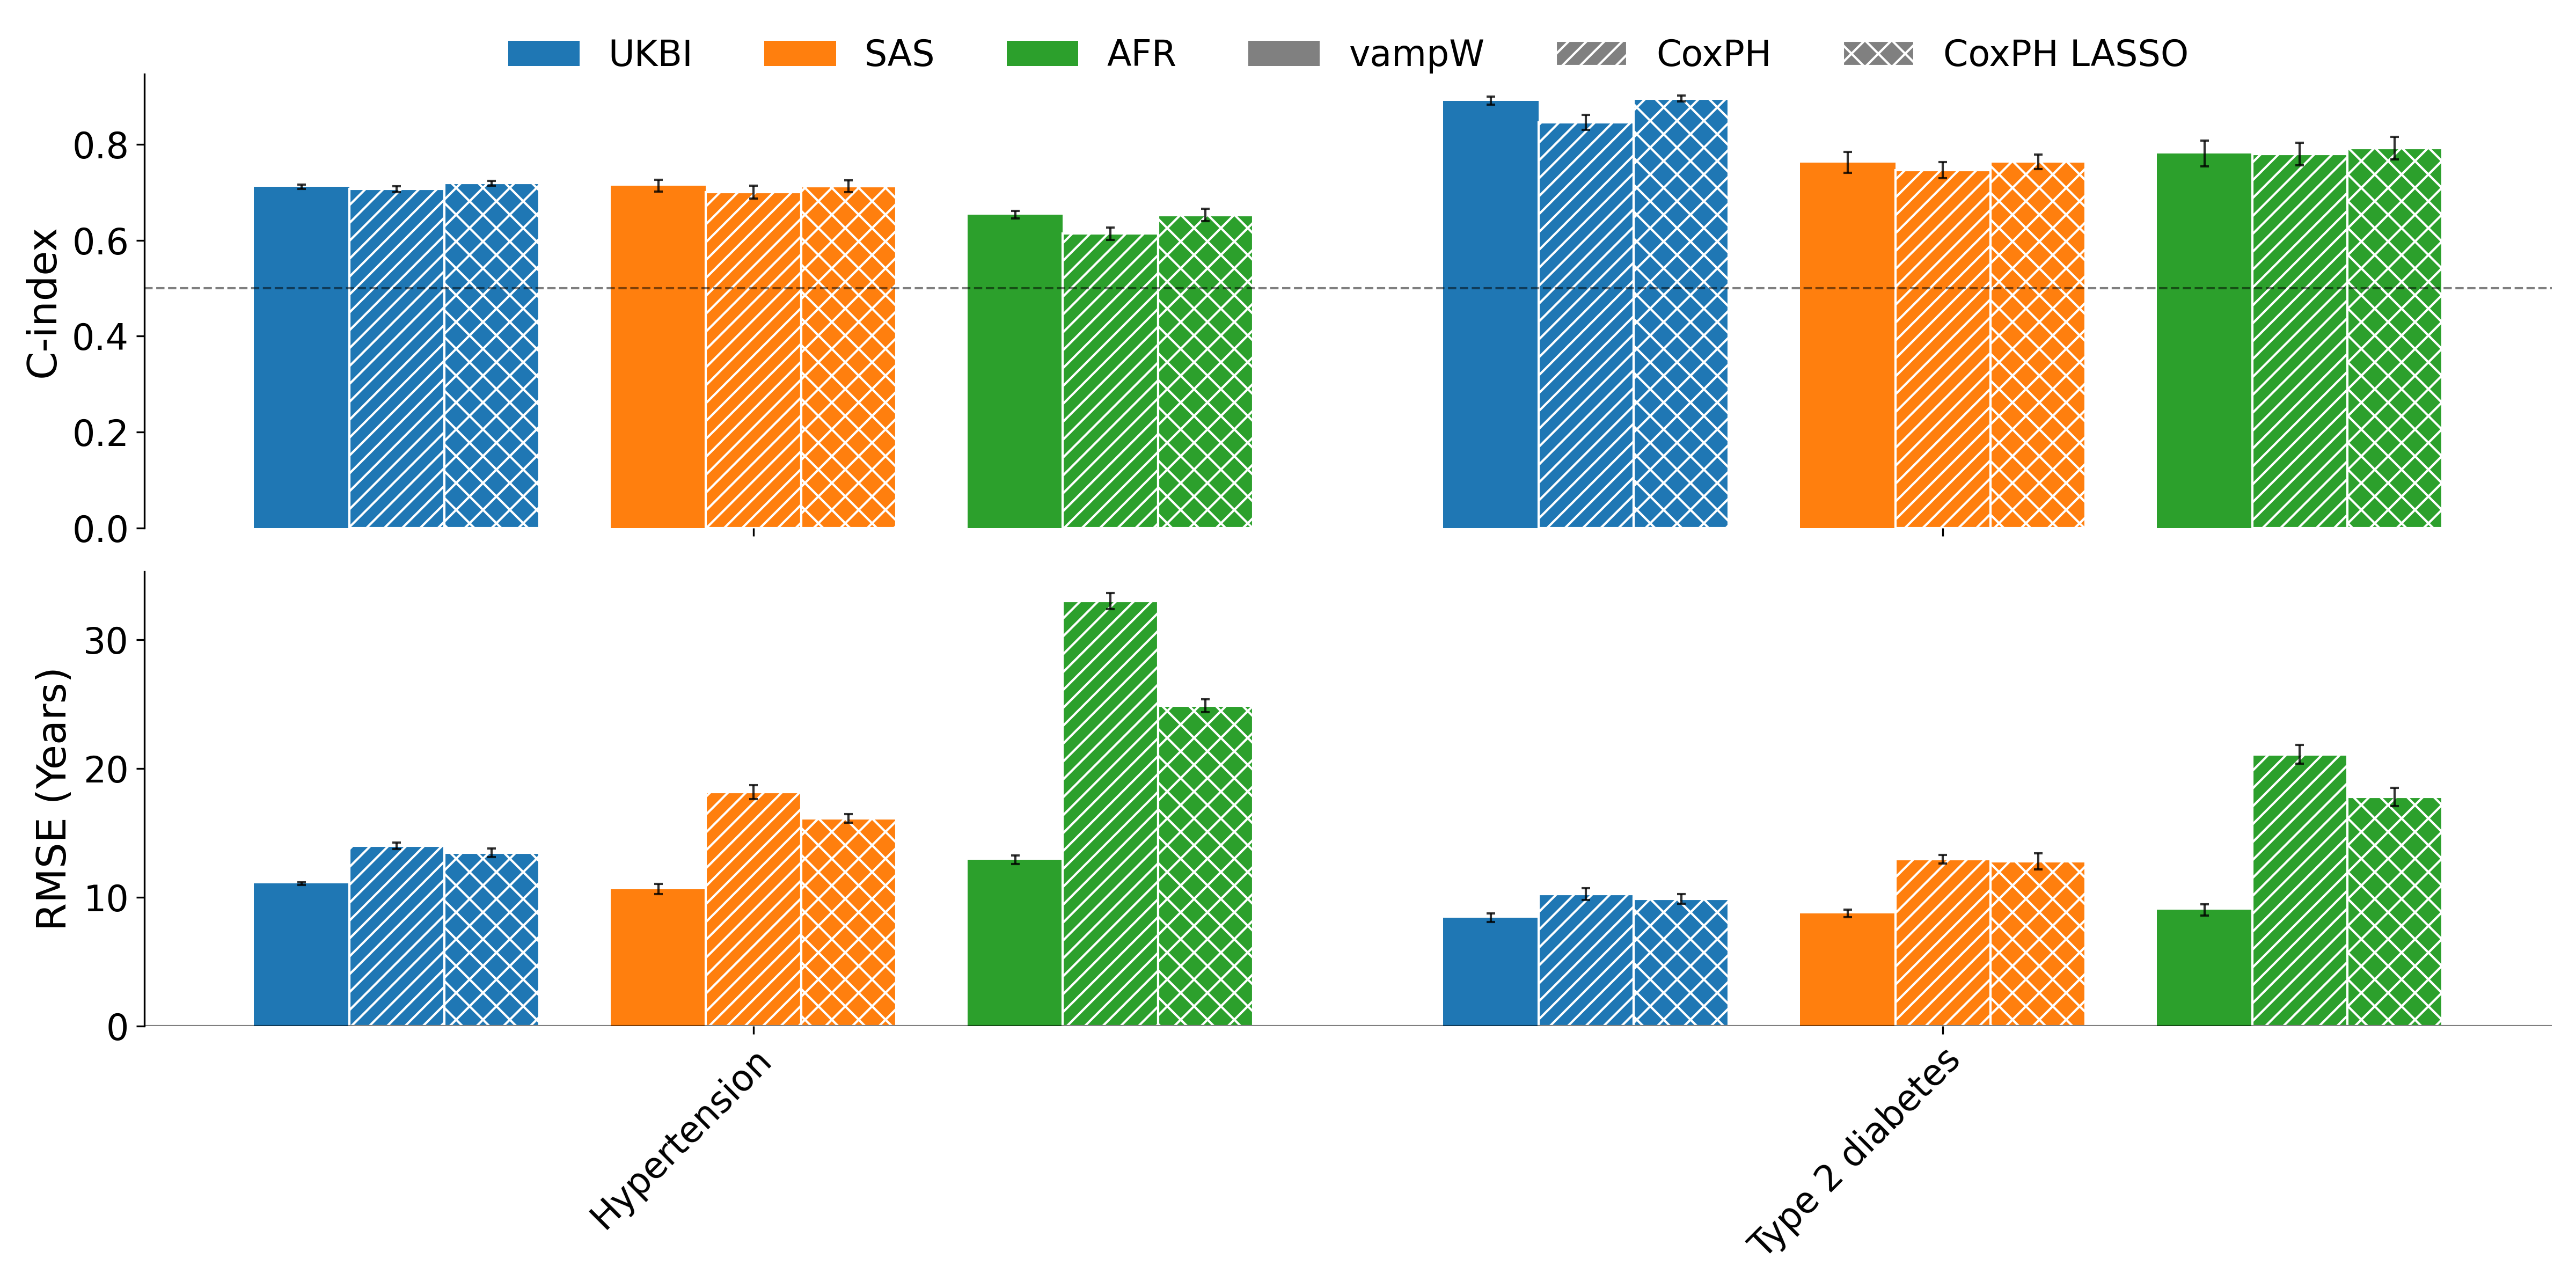
\includegraphics[width=\linewidth]{figures/genetic_ancestry_exp_50_10.png}
    \end{center}
    \caption[Out-of-sample prediction performance across distinct genetic ancestries]{\textbf{Out-of-sample prediction performance across distinct genetic ancestries.} We evaluate the predictive performance of vampW (solid bars), the standard CoxPH model (diagonal hatch lines), and CoxPH LASSO (cross hatch lines) across Hypertension and Type 2 diabetes traits from the UK Biobank. Results are stratified by genetic ancestry: British or Irish (UKBI, blue), South Asian (SAS, orange), and African (AFR, green). Performance is measured using the concordance index (C-index, top panel) and root mean squared error (RMSE in years, bottom panel). Phenotypic traits were included only if at least one minority ancestry group (SAS or AFR) contained a minimum of 200 total cases, ensuring that the 50\% data splits retained at least 100 cases per split. The reported error bars represent the standard deviation across 10 splits, with each split evaluating a random 50\% subsample of the dataset. We note that polygenic risk scores created by vampW are transferable to minority populations in the cohort; vampW exhibits similar C-index performance to Cox LASSO and outperforms the joint standard Cox model, while outperforming both competitor models in terms of the RMSE metric.}
\label{fig:genetic_ancestry_exp_50_10}
\end{figure}

\clearpage

\begin{figure}[H]
    \begin{center}
        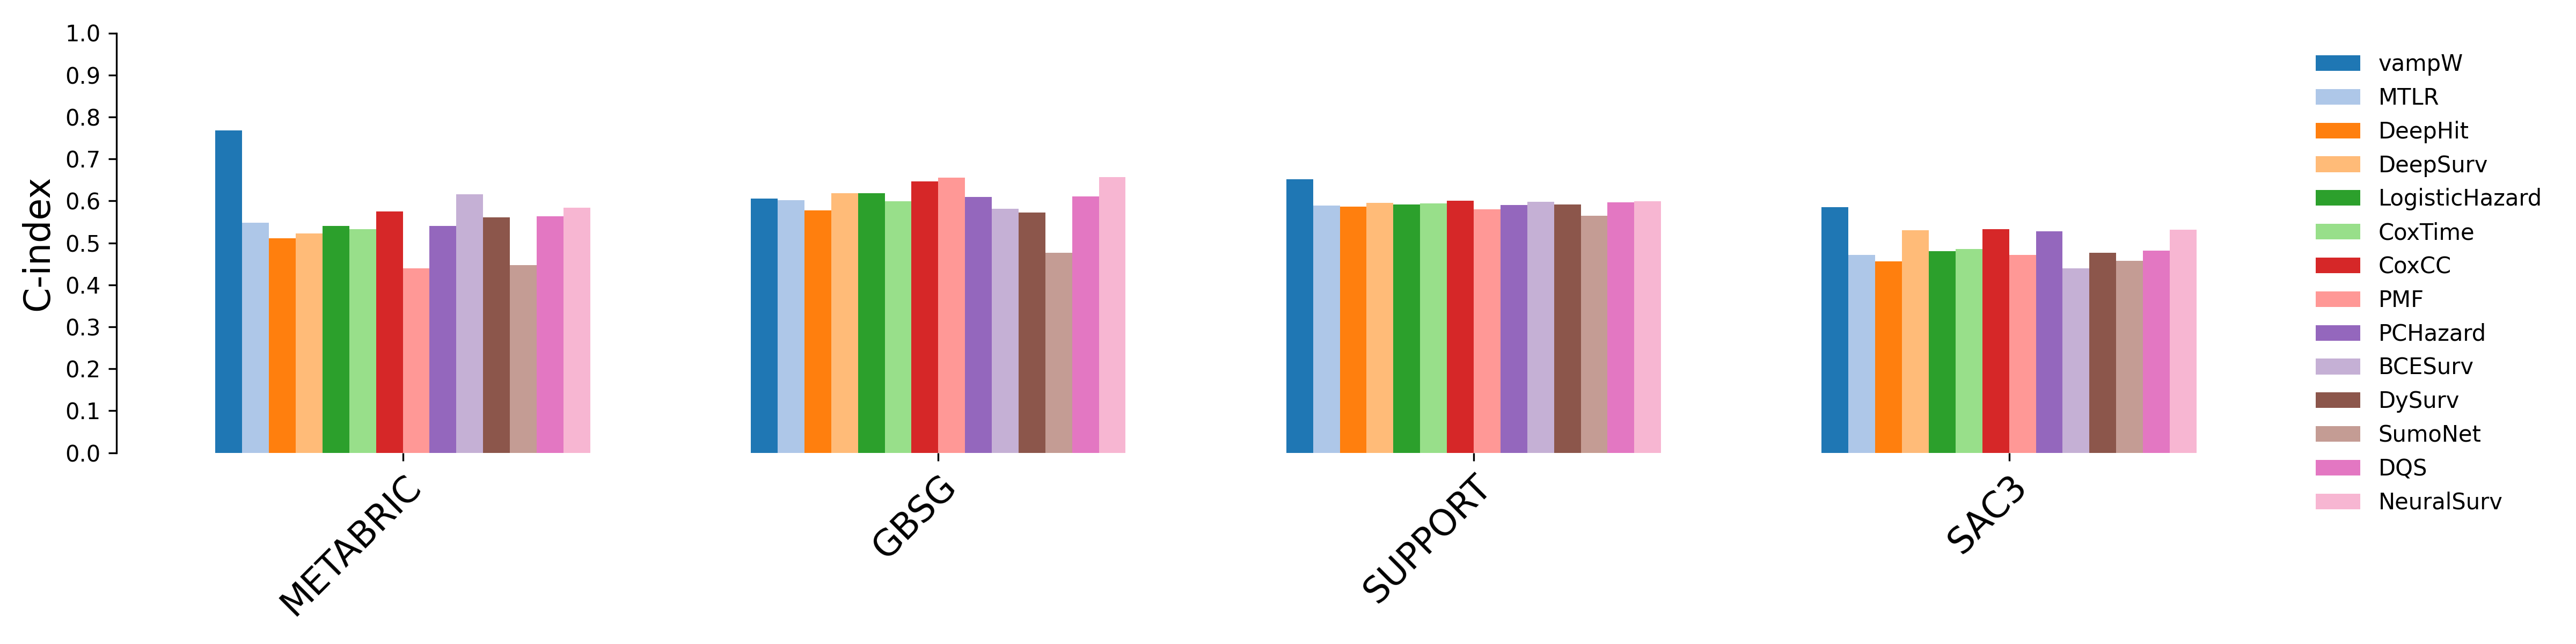
\includegraphics[width=\linewidth]{figures/deep_benchmark.png}
    \end{center}
    \caption[Out-of-sample performance comparison in terms of the Concordance index for vampW and deep learning methods]{\textbf{Out-of-sample performance comparison in terms of the Concordance index for vampW and deep learning methods.}
We compare predictions of vampW with common deep learning methods on several widely used survival benchmarking datasets, namely METABRIC, GBSG, SUPPORT, and SAC3. The benchmarking results for deep learning are reported in a recent NeuralSurv study \cite{monod_neuralsurv_2025}, which addresses prediction in data-scarce regimes. vampW outperforms all deep learning methods on METABRIC, SUPPORT, and SAC3 datasets, and outperforms 6 out of 13 benchmarking methods on the GBSG dataset.}
\label{fig:deep_benchmark}
\end{figure}

% \clearpage 


% \begin{figure}[H]
% \label{fig:vampw_age_corr}
%     \begin{center}
%         \includegraphics[width=\linewidth]{figures/real_vampw_cov_exp.png}
%     \end{center}
%     \caption{
%     \changed{\jakub{Figure added for consideration of whether to include it.}\textbf{Out-of-sample performance of vampW across two different approaches to age covariate adjustment.} We evaluate the out-of-sample C-index and Brier score at the 75\% time point for vampW, adjusting for age using either a linear model (solid color) or an exponential model (hatched color).}}
% \end{figure}

% \clearpage

% \begin{figure}[H]
% \label{fig:vampw_age_corr_disc}
%     \begin{center}
%         \includegraphics[width=\linewidth]{figures/real_vampw_disc.png}
%     \end{center}
%     \caption{
%     \changed{\jakub{Figure added for consideration of whether to include it.}\textbf{Number of vampW discoveries across different age correction approaches.} We plot number of significant proteomic markers above PIP threshold of 95\% for vampW, correcting for age using either a linear model (solid color) or an exponential model (hatched color). Here, we select the best iteration based on the highest C-index on the training data after several warm-up iterations. As the model in the exponentially corrected analysis stabilizes in later iterations, we use a longer warm-up period of 10 iterations, compared with 5 iterations in the linear approach.}}
% \end{figure}

\clearpage

% \section{Supplementary Note}
%\textbf{
\section{Details on denoiser for Weibull link function}
\label{sec:sup1}


We assume observations are independent, allowing for component-wise Maximum A Posteriori estimation. Proceeding with the construction of an age-at-onset denoiser for individual $i$, we express the posterior as follows, excluding terms independent of $z_i$:

\begin{equation}
    \begin{split}
    \arg \max_{z_i} \bigg \{ & \exp \bigg ( - \alpha z_i - y_i^{\alpha} \cdot \exp(-\alpha (\mu + z_i) - K) \bigg ) \\
    & \cdot \exp \bigg (-\frac{(z_i-p_{1, i})^2 \cdot \tau_1}{2} \bigg ) \bigg \}.
    \end{split} 
\end{equation}
Let us define $g_z: \mathbb{R} \to \mathbb{R}$ as
\begin{align}
    g_z(z_i) = -\alpha z_i - y_i^\alpha \cdot e^{-\alpha(\mu_i+z_i) - K} - \frac{(z_i-p_{1, i})^2 \cdot \tau_1}{2}.
\end{align}
Then, taking the derivative with respect to $z_i$, one obtains
\begin{equation}
     -\alpha + \alpha e^{-\alpha (\mu_i + z_i) - K} \cdot y^\alpha - \tau_{1}(z_i-p_1) = 0,
\end{equation}
which can be solved using fixed-point iterations. In addition, we note that
\begin{align}
 g_z''(z_i) = -\alpha^2 \cdot y_i^\alpha \cdot e^{-\alpha(\mu_i+z_i)-K} - \tau_1 < 0, \quad \text{for all } z_i,
\end{align}
and, hence, $g$ is a strictly concave function (see a visualization in Supplementary Figure \ref{fig:enter-label}).

\begin{figure}[!ht]
    \centering
    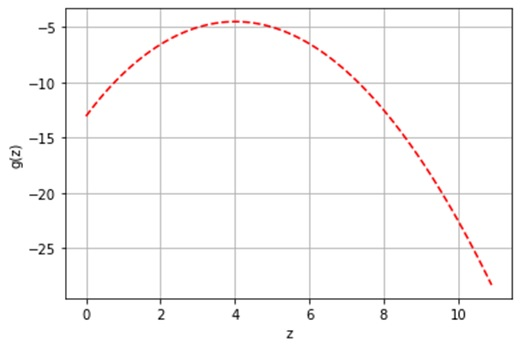
\includegraphics[width=0.44\linewidth]{figures/gz_weibull.jpg}
    \caption[Visualization of a function $g_z(z_i)$]{Visualization of a function $g_z(z_i)$ for $\alpha = 1, \tau_1 = 1, p = 5, \mu_i = 0, y_i = 1$}
    \label{fig:enter-label}
\end{figure}
Furthermore, by invoking the Implicit Function Theorem, we can compute the derivative of the denoiser as
\begin{align}
    \frac{dz}{dp_1} = \frac{\tau_1}{\tau_1 + \alpha^2 y_i^\alpha \cdot e^{-\alpha(\mu_i+z_i) - K}}.
\end{align}

\section{Details on EM hyperparameter updates}
\label{sec:sup3}

We %In this section, we 
present the derivation of the expectation-maximization update formulae for the hyperparameters $\mu$ and $\alpha$ under the Weibull model for non-censored phenotypic outcomes. We define the E-step and M-step of the EM algorithm at iteration $t$ of vampW in the following way:
\begin{enumerate}
    \item \underline{E-step}: The approximation of the posterior distribution typical for E-steps happens implicitly in VAMP-type algorithms, where the following
    approximate posterior probability distribution for the genetic component, $\bm{z} = \bm{X} \bm{\beta}$,  is obtained:
    \begin{align}
        b^{(t)}(\bm{z}) = \mathcal{N}(\bm{z}; \bm{\hat{z}_{2t}}^{(t)}, \bm{I}_N / \xi^{(t)}).
    \end{align}
    \item \underline{M-step}: We aim to maximize the evidence likelihood over $\mu$ and $\alpha$
    \begin{align}
        (\alpha^{(t+1)}, \mu^{(t+1)}) = \text{argmax}_{\mu, \alpha} \{ L^{(t)}(\mu, \alpha) \},
    \end{align}
    where we define 
    \begin{align}
        \begin{split}
        L^{(t)}(\mu, \alpha) & = \sum_{i=1}^N \int b_i^{(t)}(z_i) \cdot \log p(y_i|z_i, \alpha, \mu) dz_i \\
        & \quad = \sum_{i=1}^N \int \mathcal{N}(z_i; \hat{z}_i^{(t)}, 1 / \xi^{(t)}) \cdot \log p(y_i|z_i, \alpha, \mu) dz_i.
        \end{split}
    \end{align}
Here, $b_i^{(t)}(z_i)$ is the marginal distribution of the $i$-th component of $\bm{z}$ obtained from $b^{(t)}(\bm{z})$ and $\mathcal{N}(x; \mu, \sigma^2)$ denotes the probability density function of a Gaussian with mean $\mu$ and variance $\sigma^2$ evaluated at $x$.
    Furthermore, note that
    \begin{align}
        \begin{split}
        \log p(y_i|z_i, \alpha, \mu) & = \log(\alpha) + \alpha(\log y_i - \mu - z_i) - K \\
        & \quad - e^{\alpha(\log y_i - \mu - z_i) - K}.
        \end{split}
    \end{align}
\end{enumerate}
\underline{\textbf{Update formula for} $\alpha$:} \newline \newline
By taking the derivative of $L(\mu, \alpha)$ with respect to $\alpha$ and equating to zero we obtain:
\begin{align}
    \begin{split}
    \frac{\partial L^{(t)}(\mu, \alpha)}{\partial \alpha} = 0 & = \sum_{i=1}^N \int \mathcal{N}(z_i; \hat{z}^{(t)}, 1 / \xi^{(t)}) \cdot \left\{\frac{1}{\alpha} + \left(\log y_i - \mu - z_i\right) \right. \\
    & \qquad \left. \cdot \left[1 - e^{\alpha\left(\log y_i - \mu - z_i\right) - K}\right]\right\} dz_i.
    \end{split} 
\end{align}
Separating the term in brackets results in
\begin{align}
    \begin{split}
     & \sum_{i=1}^N \bigg [\frac{1}{\alpha} + \log y_i - \mu - \hat{z}_i^{(t)} \bigg ] \\
     &=
     \frac{N}{\alpha} + \sum_{i=1}^N [\log y_i - \mu - \hat{z}_i^{(t)}]  \\ 
     &= \sum_{i=1}^N \mathcal{N}(z_i; \hat{z}_i^{(t)}, 1 / \xi^{(t)}) \cdot (\log y_i - \mu - z_i) \cdot e^{\alpha(\log y_i - \mu - z_i) - K} dz_i \\
    &= \sum_{i=1}^N \int \mathcal{N}(\log y_i - \mu - \phi_i; \hat{z}_i^{(t)}; 1/\xi^{(t)}) \cdot \phi_i \cdot e^{\alpha \phi_i - K} d \phi_i \\
    &= e^{-K} \cdot \sum_{i=1}^N \exp(\alpha (\log y_i - \mu - \hat{z}_i^{(t)}) + \frac{\alpha^2}{2 \xi^{(t)}}) \\
    & \qquad \cdot \bigg ( (\log y_i - \mu - \hat{z}_i^{(t)}) + \frac{\alpha}{\xi^{(t)}} \bigg ).
    \end{split}
\end{align}
Finally, we define $f_{i}(\alpha) := e^{a_i \alpha + b \alpha^2 / 2} \cdot (a_i + \alpha b)$, where $a_i = \log y_i - \mu - {\hat{z}_i}^{(t)}$ and $b = \frac{1}{\xi^{(t)}}$. It follows that
\begin{align}
    f'(\alpha) = e^{a \alpha + b \alpha^2 / 2} ( a^2 + b + 2 ab \alpha + b^2 \alpha^2) > 0 \quad \text{ for all } \alpha > 0,
\end{align}
i.e. the function is strictly increasing in $\alpha$. This implies that the first derivative with respect to $\alpha$ of the likelihood function $L^{(t)}$ is
\begin{equation}
\frac{\partial L^{(t)}(\mu, \alpha)}{\partial \alpha} = \text{const} + \frac{N}{\alpha} - e^{-K} \sum_{i=1}^{N}f_i(\alpha).
\end{equation}
The second derivative is then given by

\begin{equation}
\frac{ \partial^2 L^{(t)}(\mu, \alpha)}{\partial^2 \alpha} = -\frac{N}{\alpha^2} - e^{-K} \sum_{i=1}^{N}f_i'(\alpha) < 0, \quad \mbox{for all } \alpha > 0.
\end{equation}
We thus have that the second derivative with respect to $\alpha$ is negative on the considered domain and hence the root of $\partial_{\alpha}L^{(t)}(\alpha, \mu) = 0$ attains a unique global maximum on the considered domain. We solve for the global maximizer $\alpha^*$ using numerical methods (SciPy optimize).
\newline
\newline
\noindent \underline{\textbf{Update formula for} $\mu$:} 
\newline 

\noindent Similarly, by taking the partial derivative of $L^{(t)}(\mu, \alpha)$ with respect to $\mu$ and equating it to zero, we obtain
\begin{align}
    \frac{\partial L^{(t)}(\mu, \alpha)}{\partial \mu} = 0 = \sum_{i=1}^N \int \mathcal{N}(z_i; \hat{z}_i^{(t)}, 1 / \xi^{(t)}) \cdot \alpha \cdot  [ e^{\alpha(\log y_i - \mu - z_i) - K} - 1] dz_i, 
\end{align}
where we use that 
\begin{align}
\frac{\partial \log p(y_i|z_i, \alpha, \mu)}{\partial \mu}= -\alpha + \alpha e^{\alpha(\log y_i - \mu - z_i) - K}.
\end{align}

By separating the term in brackets it follows that
\begin{align}
    \begin{split}
0 & = \alpha \sum_{i=1}^{n} \int \mathcal{N} \bigg (z_i; \hat{z}_i^{(t)}, \frac{1}{\xi^{(t)}} \bigg ) e^{\alpha(\log y_i - \mu - z_i) - K} dz_i \\
& \qquad - \alpha \sum_{i=1}^{n} \int \mathcal{N} \bigg (z_i; \hat{z}_i^{(t)}, \frac{1}{\xi^{(t)}} \bigg ) dz_i \\
& = \alpha \sum_{i=1}^{n} \exp \left( -K + \frac{\alpha^2}{2 \xi^{(t)}} + \alpha (\log y_i - \hat{z}_i^{(t)} - \mu) \right) \\
& \qquad - \alpha N \exp \left( -K + \frac{\alpha^2}{2 \xi^{(t)}} - \alpha \mu \right) \sum_{i=1}^{n} \exp \left( \alpha (\log y_i - \hat{z}_i^{(t)}) \right) \\
& = N -K + \frac{\alpha^2}{2 \xi^{(t)}} - \alpha \mu + \log \left( \sum_{i=1}^{n} \exp \left( \alpha (\log y_i - \hat{z}_i^{(t)}) \right) \right) \\
& = \log N.
    \end{split}
\end{align}
Hence, the update formula for $\mu$ satisfies
\begin{align}
\begin{split}
\mu & = \frac{-K}{\alpha} + \frac{\alpha}{2 \xi^{(t)}} \\
& \quad + \frac{1}{\alpha} \log \left( \sum_{i=1}^{n} \exp \left( \alpha (\log y_i - \hat{z}_i^{(t)}) \right) \right) - \frac{1}{\alpha} \log N.
\end{split}
\end{align}

Furthermore, the maximization problem at hand is concave: 
% We are considering maximization with respect to \(\alpha\) \marco{$\mu$?}:

% \[
% \text{argmax}_{\mu} \left\{ \sum_{i=1}^{N} \int \mathcal{N}(z_i; \hat{z}^{(t)}, 1 / \xi^{(t)}) \cdot \log p(y_i|z_i, \alpha, \mu) \, dz_i \right\} = \text{argmax}_{\mu} \{L(\mu)\}
% \]

% \[
% \frac{\partial L}{\partial \mu} = \exp \left( -K + \frac{\alpha^2}{2 \xi^{(t)}} - \alpha \mu \right) \sum_{i=1}^{n} \exp \left( \alpha (\log y_i - \hat{z}_i^{(t)}) \right) - N
% \]
\begin{equation}
\begin{split}
\frac{\partial^2 L^{(t)}}{\partial \mu^2} & = - \alpha \exp \left( -K + \frac{\alpha^2}{2 \xi^{(t)}} - \alpha \mu \right) \\
& \qquad \sum_{i=1}^{n} \exp \left( \alpha (\log y_i - \hat{z}_i^{(t)}) \right) - N < 0 \quad \text{for all } \alpha > 0.
\end{split}
\end{equation}

Therefore, $\mu$ satisfying $\frac{\partial L^{(t)}}{\partial \mu} = 0$ attains the global maximum of $L^{(t)}(\mu)$. 
%\marco{I did not understand the point of a few formulas above so I have removed them. Please restore in case I misunderstood the argument.} % in terms of $\mu$.

\clearpage

\section{Details on non-linear MMSE handling right-censorship}
\label{sec:sup2}

\noindent 
\begin{lemma}
    Differentiating the function inside the optimization problem (\ref{formula:cenosring_opt_problem}) with respect to $\bm{\beta}$ and equating the result to zero yields 
    \begin{align}
    %\nabla_\beta \text{nll} = 
    \begin{split}
    & 2 \gamma_{2t} (\bm{\beta} - \bm{r}_{2t}) + 2 \tau_{2t} \bm{X}^\top(\bm{X}\beta - \bm{p}_{2t}) \\
    & \quad - \alpha \bm{X}_\mathcal{C}^\top h(\alpha(\log(\bm{y}_\mathcal{C}) - \mu - \bm{X}_\mathcal{C} \bm{\beta})-K)= 0,
    \end{split}
    \end{align}
    where $h:\mathbb{R} \to \mathbb{R}$ is the standard hazard function of the Gumbel model given by $h(x) = e^x$, and the notation h($\bm{v}$) with $\bm{v}\in \mathbb{R}^{N}$ denotes the component-wise application of the function $h$. Furthermore, the Onsager corrections for the denoiser and nonlinear MMSE step are equal to 
\begin{align}
    \begin{split}
    \alpha_{2t} & = \frac{2 \cdot \gamma_{2t} \cdot \text{Trace}([J_{\beta}F(\hat{\bm{\beta}}_{2t})]^{-1})}{P}
    \quad \text{and} \\
    \upsilon_{2t} & = \frac{2 \cdot \tau_{2t} \cdot \text{Trace}(\bm{X} \cdot [J_{\beta}F(\hat{\bm{\beta}}_{2t})]^{-1} \cdot \bm{X}^\top)}{N}.
    \end{split}
\end{align}
\end{lemma}

\begin{proof}
    Let us define the function $g: \mathbb{R}^P \to \mathbb{R}$ with
    \begin{align}
    g(\bm{\beta}) = - \sum_{i=1}^{N_{\mathcal C}} \log S(\alpha(\log(y_{c,i}) - \mu - (\bm{X}_\mathcal{C} \bm{\beta})_i) -K),
    \end{align}
    where $N_{\mathcal C}$ is the number of censored individuals in the study and $\bm{X}_{\mathcal C}$ is the design matrix corresponding to those individuals. By performing differentiation, it follows that
    \begin{align}
        \begin{split}
        \frac{\partial g(\bm{\beta})}{\partial \bm{\beta}_j} & = - \sum_{i=1}^{N_{\mathcal C}} \alpha \cdot h(\alpha(\log(y_{c,i}) - \mu - (\bm{X}_\mathcal{C} \bm{\beta})_i) - K) \cdot  (\bm{X}_{\mathcal C})_{i,j} \\ & = - \alpha \langle h(\alpha(\log(y_{c,i}) - \mu - (\bm{X}_\mathcal{C} \beta)_i) - K), (\bm{X}_{\mathcal C})_{:,j} \rangle.
        \end{split}
    \end{align}
    Hence,
    \begin{align}
        \nabla_{\bm{\beta}} g(\bm{\beta})  = - \alpha \cdot \bm{X}_{\mathcal C}^\top h(\alpha(\log(\bm{y}_\mathcal{C}) - \mu - \bm{X}_\mathcal{C} \bm{\beta}) - K).
    \end{align}
    Furthermore,
    \begin{align}
        \begin{split}
        \frac{\partial g(\bm{\beta})}{\partial \bm{\beta}_k \partial \bm{\beta}_j} & = \frac{\partial}{\partial \bm{\beta}_k} \bigg [ - \sum_{i=1}^{N_{\mathcal C}} \alpha \cdot h(\alpha(\log \bm{y}_\mathcal{C} - \mu - \bm{X}_\mathcal{C} \bm{\beta})-K) \cdot (\bm{X}_{\mathcal C})_{i,j} \bigg ] \\
        & = \alpha^2 \sum_{i=1}^{N_{\mathcal C}} h'(\alpha (\log y_{c,i} - \mu - (\bm{X}_\mathcal{C} \bm{\beta})_i) - K) \cdot (\bm{X}_{\mathcal C})_{i,j} \cdot (\bm{X}_{\mathcal C})_{i,k} \\
        & = \alpha^2 \langle h'(\alpha (\log y_{c,i} - \mu - (\bm{X}_\mathcal{C} \bm{\beta})_i) - K) \cdot (\bm{X}_{\mathcal C})_{:,j}, (\bm{X}_{\mathcal C})_{:,k} \rangle,
        \end{split}
    \end{align}
    with $h'(x) = e^x$.
    It directly follows that
    \begin{align}
        \nabla^2 g(\bm{\beta}) = \alpha^2 \bm{X}_\mathcal{C}^\top \text{Diag}(h'(\alpha(\log \bm{y}_\mathcal{C} - \mu - \bm{X}_\mathcal{C} \bm{\beta})-K)) \bm{X}_\mathcal{C}.
    \end{align}
    We now define $F:\mathbb{R}^P \to \mathbb{R}^P$ as
    \begin{align}
        F(\beta) = 2(\gamma_{2t}\bm{I} + \tau_{2t}\bm{X}^\top\bm{X}) \bm{\beta} - \alpha \bm{X}_\mathcal{C}^\top h(\alpha(\log(\bm{y_\mathcal{C}}) - \mu - \bm{X_\mathcal{C}} \bm{\beta})-K),
    \end{align}
    which means that a solution $\hat{\bm{\beta}}_{2t}$ to the optimization problem (\ref{formula:cenosring_opt_problem}) satisfies 
    
    \begin{align}
        \hat{\bm{\beta}}_{2t} = F^{-1}(2 \gamma_{2t} \bm{r}_{2t} + 2 \tau_{2t} \bm{X}^\top \bm{p}_{2t}).
    \end{align}
    Note that
    \begin{align}
        \begin{split}
        & \text{div}_{r_{2t}}( F^{-1}(2 \gamma_{2t} r_{2t} + 2 \tau_{2t} \bm{X}^\top \bm{p}_{2t}) ) \\
        & = \text{Trace}(J_{\beta}F^{-1}(2 \gamma_{2t} r_{2t} + 2 \tau_{2t} \bm{X}^\top \bm{p}_{2t})) \cdot 2 \gamma_{2t} \\
        & = \text{Trace}([J_{\beta}F(F^{-1}(2 \gamma_{2t} r_{2t} + 2 \tau_{2t} \bm{X}^\top \bm{p}_{2t}))]^{-1}) \cdot 2 \gamma_{2t} \\
        & = \text{Trace}([J_{\beta}F(\hat{\bm{\beta}}_{2t})]^{-1}) \cdot 2 \gamma_{2t},
        \end{split}
    \end{align}
    where 
    \begin{align}
        \begin{split}
        J_{\beta} F(\hat{\beta}_{2t}) & = 2(\gamma_{2t}I + \tau_{2t}\bm{X}^\top\bm{X}) + \nabla^2 g(\hat{\bm{\beta}}_{2t}) \\
        & = 2(\gamma_{2t}I + \tau_{2t}\bm{X}^\top\bm{X}) \\
        & \qquad + \alpha^2 \bm{X}_\mathcal{C}^\top \text{Diag}\big(h'(\alpha(\log \bm{y}_\mathcal{C} - \mu - \bm{X}_\mathcal{C} \hat{\bm{\beta}}_{2t})-K)\big) \bm{X}_\mathcal{C}.
        \end{split}
    \end{align}
    Finally, we conclude that % Onsager correction for $\bm{\beta}$-denosier is
    \begin{align}
        \alpha_{2t} = \frac{2 \cdot \gamma_{2t} \cdot \text{Trace}([J_{\beta}F(\hat{\bm{\beta}}_{2t})]^{-1})}{P}.
    \end{align}
    Similarly, we derive %now proceed to deriving the Onsager correction for $z$:
    \begin{align}
        \begin{split}
        & \text{div}_{p_{2t}}(\bm{X} F^{-1}(2 \gamma_{2t} \bm{r}_{2t} + 2 \tau_{2t} \bm{X}^\top \bm{p}_{2t}) ) \\
        & = \text{Trace}(\bm{X} J_{\beta}F^{-1}(2 \gamma_{2t} \bm{r}_{2t} + 2 \tau_{2t} \bm{X}^\top \bm{p}_{2t}) \cdot 2 \tau_{2t} \cdot \bm{X}^\top) \\
        & = \text{Trace}(\bm{X} [J_{\beta}F(F^{-1}(2 \gamma_{2t} \bm{r}_{2t} + 2 \tau_{2t} \bm{X}^\top \bm{p}_{2t}))]^{-1} \cdot 2 \tau_{2t} \cdot \bm{X}^\top) \\
        & = 2 \tau_{2t} \cdot \text{Trace}(\bm{X} \cdot [J_{\beta}F(\hat{\beta}_{2t})]^{-1} \cdot \bm{X}^\top),
        \end{split}
    \end{align}
    which gives the Onsager correction %
%    Finally, we conclude the Onsager correction for $z$:
    \begin{align}
        \upsilon_{2t} = \frac{2 \cdot \tau_{2t} \cdot \text{Trace}(\bm{X} \cdot [J_{\beta}F(\hat{\bm{\beta}}_{2t})]^{-1} \cdot \bm{X}^\top)}{N}.
    \end{align}
    \end{proof}

\clearpage

\section{Details on Weibull and ExpGamma outcomes} \label{sec:sup4}

For the Weibull model, %given the $\bm{\beta}$ vector is already drawn as described in Methods \ref{sec:methods_sim}, 
we calculate the scaling factor 
\begin{equation}
    c = \sqrt{\bigg (\frac{1}{\sigma^2_G} - 1 \bigg ) \cdot \frac{\text{Var}(\bm{X}\bm{\beta})}{\sigma^2_{w}}},
\end{equation}
where $\sigma^2_w=\pi^2/6$ is the variance of the Gumbel distribution. Then, we generate time-to-event phenotypes as:
\begin{equation}
    \log({\bm{y}}) = \mu + \bm{X}\bm{\beta} + c \cdot (\bm{w} + \kappa).
\end{equation}
This formulation means that, in the phenotype $\log(\bm{y})$, the targeted proportion of variance is explained by markers.

For ExpGamma-distributed phenotypes, we exploit the fact that if $x \sim \text{ExpGamma}(\kappa, \theta, \tilde{\mu})$, then $ax + b \sim \text{ExpGamma}(\kappa, a \theta, a \tilde{\mu} + b)$. Then, we rewrite the model as follows:
\begin{align}
    \log y_i = \mu + \bm{x}_i^\top \bm{\beta} + \theta(w_i - \psi^{(0)}(\kappa)), \quad w_i \sim \text{ExpGamma}(\kappa, 1, 0),
\end{align}
with shape parameter $\kappa$, scale parameter $\theta$, and location parameter $\mu$.  We note that
\begin{align}
    \begin{split}
    & \mathbb{E}[\log y_i] = \theta  \psi ^{(0)}(\kappa )+ \tilde{\mu}, \\
    & 
    \text{Var}[\log y_i] = \theta ^2 \psi ^{(1)}(\kappa ),
    \end{split}
\end{align} where $\psi^{(m)}(\cdot)$ stands for the polygamma function of order $m$. Using the parametrization
\begin{equation}
    \theta = \sqrt{\bigg (\frac{1}{\sigma^2_G} - 1 \bigg ) \cdot \frac{\text{Var}(\bm{X\beta}) }{ \psi^{(1)}(\kappa)}},
\end{equation}
we obtain the time-to-event phenotypic outcomes, with the desired proportion of variance explained by the simulated markers.

\clearpage
